\chapter{Аналіз та ідентифікація фізичної реалізації системи Колпітца}
\label{atu:ch:colpreal}

\LinkRef{
  colp: ASAU-21, APIR-2013
}

\section{Визначення системи}%%{{{1
\label{atu:s:colp_task}


У ряді радіоелектронних пристроїв використовуються генератори
сигналів, здатні генерувати різноманітні види сигналів, в тому
числі складно-періодичні та хаотичні~\cite{dmitriev_gen_chaos}. Зокрема,
генератор Колпітца~\cite{kennedy_chaos_colpitts,atu_asau21,Kennedy_Colpitts_predicting}, який,
в залежності від умов, може генерувати коливання, як близькі
до гармонійних, так і проявляти хаотичну динаміку в широкому
спектральному діапазоні. Ідентифікація параметрів розглянутого
генератора необхідна, з одного боку, для забезпечення необхідних
режимів роботи. З іншого боку, інформація про параметри системи
необхідна при проведенні контролю працездатності в процесі
експлуатації пристрою~\cite{atu_apir2013}.

Існує множина фізичних реалізацій генератора Колпітца. Історично
першими були схеми на електронних лампах. У теперішній час роль
активного нелінійного елемента в генераторі найчастіше виконує
біполярний або польовий транзистор~\cite{doi:10.1063/1.4705999}. Частина
сучасних робіт присвячені дослідженню генератора Колпітца на
основі мемрістора~\cite{DBLP:journals/corr/WangWQ15}. Існують загальні
явища, характерні як для генератора Колпітца, так і для
системи Чуа~\cite{Kennedy_Colpitts_Chua}.


На рис.~\ref{atu:f:colp_schem} приставлена одна з електричних схем,
що реалізують генератор Колпітца на біполярному транзисторі. З
множини схем, дана була обрана через наявність одного джерела
напруги і простоти схемотехнічної реалізації генератора.


\begin{figure}[htb!]
\begin{center}
% vi:syntax=tex

\begin{circuitikz}[line width=0.7]
  \ctikzset{bipoles/thickness=2}
  \def\Top{8.0}
  %
  \draw (3.0,3.0) node[npn](npn) {};
  \draw (2.8,3.0) circle[radius=0.5];
  %\draw (npn.center) circle[radius=0.5];
  %
  \draw (0.0,0.0)
   to[R,l=$R_2$,-*]  (0.0,3.0)
   to[R,l=$R_1$]     (0.0,\Top)
   to[short]         (6.0,\Top)
   to[battery,l=$V_{cc}$] (6.0,0.0)
   -- (0.0,0.0);
  %
  \draw (1.5,0.0) to[C,l=$C_0$,*-*] (1.5,3.0);
  \draw (0.0,3.0) -- (npn.base);
  \draw (3.0,0.0) to[vR,l=$R_e$,*-*] (3.0,2.0)
   to[short] (npn.emitter);
  \draw (npn.collector)
   to[L,l=$L$,i<=$I_L$] (3.0,6.0)
   to[R,l=$R_c$] (3.0,\Top);
  %
  \draw (4.5,0.0) to[C,l=$C_2$,v=$V_2$,*-*] (4.5,2.0);
  \draw (4.5,2.0) -- (3.0,2.0);
  \draw (4.5,2.0) to[C,l=$C_1$,v=$V_1$]     (4.5,4.0);
  \draw (4.5,4.0) -- (3.0,4.0);
  \filldraw (3.0,4.0) circle[radius=0.05];
\end{circuitikz}



%\begin{tikzpicture}[circuit ee IEC,very thick,circuit symbol unit=2.5mm]
%%\tikzset{circuit declare symbol=transistor}
%%\tikzset{set transistor graphic=transistor IEC graphic}
%  \node (R2)    at (0.0,0.0) [elelem,point up,resistor={info = $R_2$}] {};
%  \node (pR1R2) at (0.0,1.5) [contact] {};
%  \node (R1)    at (0.0,3.0) [elelem,point up,resistor={info = $R_1$}] {};
%  %
%  \node (C0)    at (1.5,0.0) [point up,elelem,capacitor={info = $C_0$}] {};
%  \node (pR2C0) at (1.5,1.5) [contact] {};
%  %
%  \node (Re)    at (3.0,0.0) [elelem,point up,resistor={adjustable,info = $R_e$}] {};
%  %\node (Q1)    at (3.0,1.5) [elelem,point right,transistor] {};
%  \node (L)     at (3.0,3.0) [elelem,point up,inductor={info = $L$}] {};
%  \node (Rc)    at (3.0,4.5) [elelem,point up,resistor={info = $R_c$}] {};
%  %
%  \node (C2)    at (4.5,0.0) [point up,elelem,capacitor={info = $C_2$}] {};
%  \node (C1)    at (4.5,3.0) [point up,elelem,capacitor={info = $C_1$}] {};
%  %
%  \node (Bat)   at (6.0,0.0) [point up,elelem,battery={info = $Vcc$}] {};
%\end{tikzpicture}


\end{center}
\caption{Електрична схема генератора Колпітца на біполярному транзисторі}
\label{atu:f:colp_schem}
\end{figure}

При створенні моделі генератора Колпітца систему рівнянь можна
заздалегідь спростити, якщо помітити, що дільник на резисторах
$\mathrm{R}_1 $,
$\mathrm{R}_2 $, разом з конденсатором
$\mathrm{C}_0 $ забезпечують сталість потенціалу бази
$V_b = V_{CC} \frac{R_1}{R_1 + R_2} $, тому з подальшого розгляду дані елементи
можна виключити.

Розглянувши процеси заряду конденсаторів і зміна струму через
котушку індуктивності~\cite{zaeplnii_radio_calc}, отримаємо наступну
систему рівнянь:
%
\begin{equation}
\label{atu:eq:colp_phys}
\begin{dcases}
  C_1 \od{V_{1}}{t}  = I_L - I_{CE} , \\
  L\, \od{I_L}{t} \; = V_{CC} - V_{1} - V_{2} - I_L R_C , \\
  C_2 \od{V_{2}}{t}  = I_L - \frac{V_{2}}{R_e}.
\end{dcases}
\end{equation}
%
%
%\noindent
де
$V_{CC} $ --- напруга живлення,
$V_1 $, $ V_2 $ --- різниця потенціалів між виводами конденсаторів
$\mathrm{C}_1 $ і
$\mathrm{C}_2 $ відповідно,
$I_L $,
$I_{CE} $ --- струми котушки індуктивності і транзистора (колектор-емітер).


Перейдемо до безрозмірних величин. При переході до
безрозмірного вигляду слід визначити, які фізичні параметри
визначають безрозмірні величини. Це необхідно для синтезу
критерію ідентифікації. Для спрощення розгляду, не знижуючи
спільності, будемо вважати
$C_1 = C_2 = C $.

Перш за все, скористаємося тим, що система містить тільки
один активний нелінійний компонент --- транзистор. Отже, саме
цей елемент визначає масштаб по напрузі. У простій моделі
транзистора такої масштабної величиною може служити
$V_{je} $ --- падіння напруги на переході база--емітер в активному
режимі. Отже, все різниці потенціалів в схемі можна нормувати
на цю величину.

Динамічні властивості (в тому числі умови початку генерації
і переходу в хаотичний режим) визначаються співвідношенням
активних і реактивних властивостей системи. При цьому величина
$\rho = \sqrt{L/C} $ має розмірність опору і визначає величину
реактивного опору. Цю величину можна використовувати для
приведення активних опорів до безрозмірного вигляду.

Для приведення струмів до безрозмірного вигляду, з урахуванням
вже обраних величин, слід використовувати величину
$V_{je} / \rho $.


Виходячи з усього перерахованого вище, позначимо:
%
\[
  x = \frac{V_{1}}{V_{je}} ; \quad
  y = \frac{\rho I_L}{V_{je}} ; \quad
  z = \frac{V_{2}}{V_{je}}, \quad
  i_{ce} = \frac{\rho I_{ce}}{V_{je}}, \quad
  c = \frac{V_{CC}}{V_{je}}, \quad
  e = \frac{V_{b}}{V_{je}}.
\]
%
\[
  b = \frac{R_c}{\rho}; \quad
  d = \frac{\rho}{R_e}. % sic!
\]

Система рівнянь набуває вигляду:
%
\begin{equation}
\label{atu:eq:colp_phys2}
\begin{dcases}
  \od{x}{t}  = \dfrac{1}{\rho C}  y - \dfrac{1}{\rho C} i_{ce} , \\
  \od{y}{t}  = \dfrac{\rho}{L} c    - \dfrac{\rho}{L} r_c y - \dfrac{\rho}{L} x- \dfrac{\rho}{L} z, \\
  \od{z}{t}  = \dfrac{1}{\rho C}  y - \dfrac{1}{\rho C} \dfrac{1}{r_e} z.
\end{dcases}
\end{equation}

Загальний множник
$\frac{1}{\rho C} = \frac{\rho}{L} = \sqrt{\frac{1}{LC}} $ в правих частинах рівнянь
природним чином задає масштаб за часом. Це підкреслює,
що частотні характеристики розглянутого генератора, на
відміну, наприклад, від релаксаційного, визначаються ємністю і
індуктивністю, тому масштаб часу задаємо так:
$T_s = \sqrt{L C} $. Тоді безрозмірний час
$t_s $ і відповідні похідні будуть визначатися як:
%
\[
  t_s = \frac{t}{T_s}; \quad
  \mathrm{d}\, t = T_s \mathrm{d}\, t_s; \quad
  \od{}{t}  = \frac{1}{T_s} \od{}{t_s}; \quad
  \od{x}{t_s} \equiv \dot{x} = T_s \od{x}{t} .
\]

Для оцінки параметрів генератора Колпітца також
використовується метод синхронізації хаотичних
коливань~\cite{PhysRevE.80.016201,picovskii_syncro,bonetti_super_persistent_colpitts}, але в даній
роботі акцент зроблений на інші методи.

% }}}1

\section{Класична модель генератора Колпітца}  % {{{1

Поведінка величини
$I_{ce} $ (надалі просто
$I_c $) досить добре описує модель Еберса-Молла~\cite{horowitz}. На жаль,
при моделюванні генератора Колпітца в літературі, присвяченій
хаотичної динаміці, використовують найпростішу модель
транзистора, вважаючи, що перехід база--емітер відкривається при
$V_{BE} = V_{je} $,
$I_c \gg I_b $, а струм колектора
%
\begin{equation}
I_c =
  \begin{cases}
    \alpha ( V_b - V_e - V_{je} ), & V_b - V_e > V_{je} \\
    0                              & \text{otherwise}.
  \end{cases}
  \label{atu:eq:bjt_libear_model}
\end{equation}


Для оцінки адекватності моделювання, в також придатності
такої класичної спрощеної моделі, в першу чергу розглянемо
модель системи з нелінійної частиною виду~(\ref{atu:eq:bjt_libear_model}). З
урахуванням усього вищевикладеного отримуємо наступну систему
рівнянь:
%
\begin{equation}
\label{atu:eq:colp}
\begin{cases}
  \dot{x} = y - a F(z), \\
  \dot{y} = c - x - by - z, \\
  \dot{z} = y - d z.
\end{cases}
\end{equation}

При цьому параметр
$b $ характеризує співвідношення активного і реактивного опору,
і, отже, режим роботи генератора. Величиною цього параметра
найпростіше управляти, змінюючи
$R_c $. Метою задачі ідентифікації буде визначення значення
цього параметра.



% }}}1

\section{Фізична реалізація генератора Колпітца} %{{{1

Для попередньої перевірки адекватності даної моделі був
створений фізичний генератор Колпітца.

На рис.~\ref{atu:f:colp_schem_real} представлена електрична схема
реалізації генератора Колпітца, яка була використана в даній
роботі. Відмінності від схеми, представленої на рис.~\ref{atu:f:colp_schem},
не принципові з точки зору моделі, і призначені як для спрощення
підключення вимірювальних пристроїв, так і для забезпечення
стабільності певних потенціалів схеми.

\begin{figure}[htb!]
\centerline{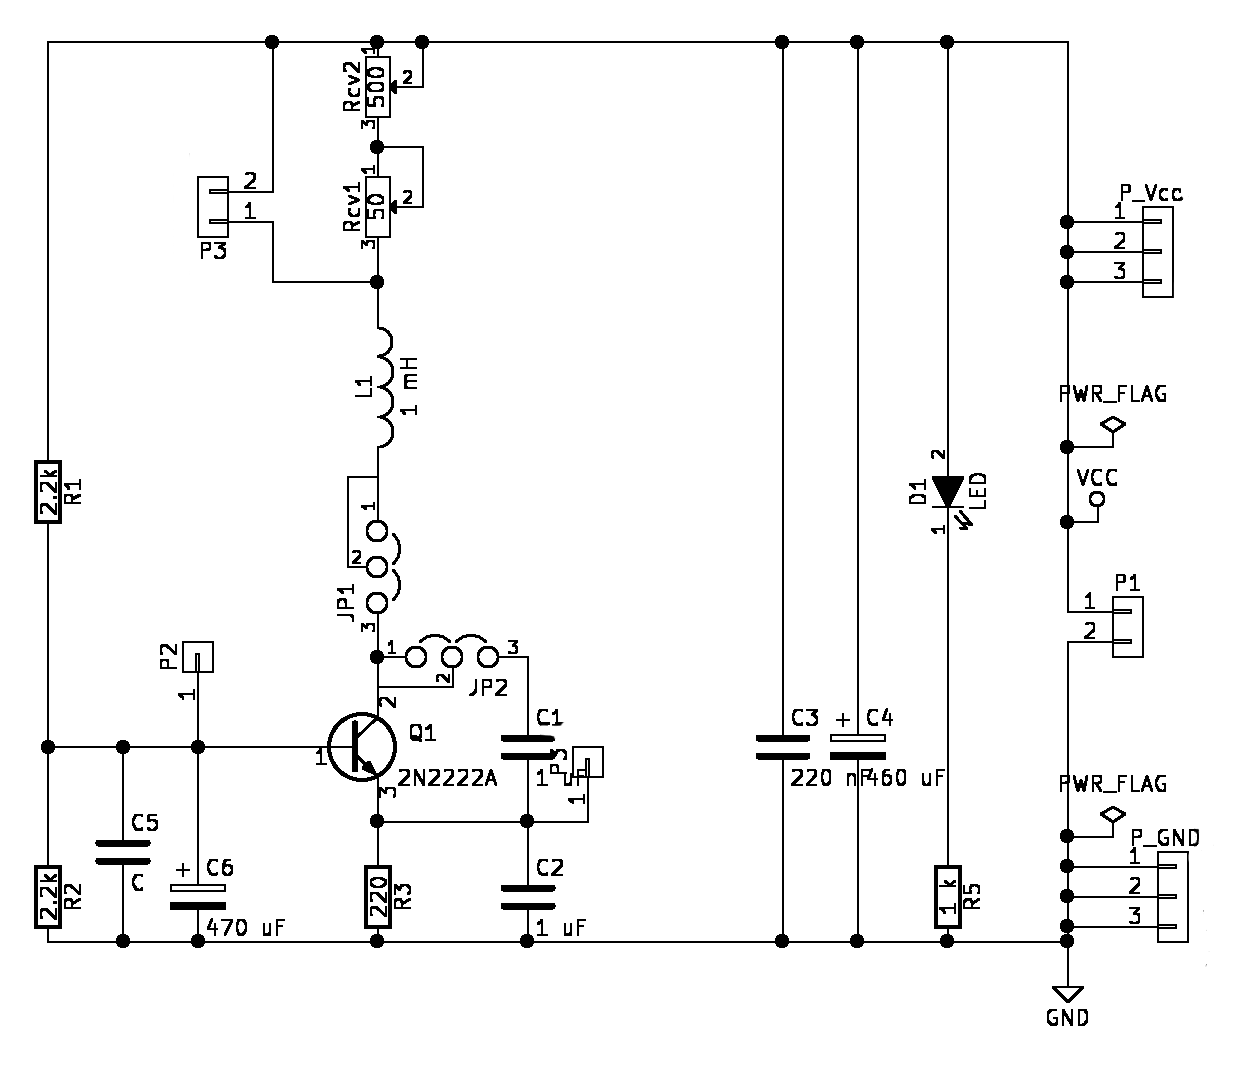
\includegraphics[width=0.8\textwidth]{p/colp_schem_real.png} }
\caption{Електрична схема генератора Колпітца, яка була використана у роботі}
\label{atu:f:colp_schem_real}
\end{figure}

Для стабілізації потенціалів
$V_{cc} $ і
$V_b $ в широкому діапазоні частот використовувалися пари
конденсаторів, відповідно
$\mathrm{C}_3$,
$\mathrm{C}_4$ і
$\mathrm{C}_5$,
$\mathrm{C}_6$. Конденсатор більшої ємності був електролітичний,
меншою --- з керамічним діелектриком. Безпосередньо в моделі
такої зміна схеми відображення не знаходить. Навпаки, ці зміни
дозволяють з меншими припущеннями вважати в моделі вищезгадані
потенціали постійними.

Резистор з базової схеми
$\mathrm{R}_c $, в реальній схемі представлений двома змінними резисторами
$\mathrm{R}_{cv1} $ і $ \mathrm{R}_{cv2} $.
Це дозволяє отримати як широкий діапазон значень
$\mathrm{R}_c $, так і можливість тонкої настройки. Слід зазначити,
що в повний опір
$\mathrm{R}_c $ входить і активний опір котушки індуктивності
$\mathrm{L}_{1} $.


Роз'єми
$\mathrm{P}_1 $,
$\mathrm{P}_\mathrm{gnd} $ і
$\mathrm{P}_\mathrm{Vcc} $ призначені для забезпечення електричним
живленням як самого генератора, так і інших приладів, які беруть
участь у вимірі. Роз'єм
$\mathrm{P}_4 $ призначений для отримання сигналу
$V_e (t) $. Роз'єм
$\mathrm{P}_2 $ дозволяє контролювати стабільність потенціалу
$V_b $, проте, в процесі вимірювання цей сигнал не записувався. Роз'єм
з набором перемичок
$\mathrm{Jp}_2 $, в першу чергу, використовується для отримання сигналу
$V_c $. Крім цього, він дозволяє відключити від схеми конденсатор
$\mathrm{C}_1 $, тим самим припинити генерацію і вивчати поведінку
схеми в стаціонарному стані для уточнення параметрів.

Роз'єм з набором перемичок
$\mathrm{Jp}_1 $ також виконує кілька функцій. Прибравши з нього
перемичку, можна виміряти повне опір
$\mathrm{R}_{c} $, що дає можливість порівняти результат ідентифікації
з реальним значенням. Також важливою властивістю є можливість
за допомогою цього роз'єму замінити пару
$\mathrm{R}_{c} $,
$\mathrm{L}_{1} $ на іншу, що розширює можливості експерименту.


Роз'єм
$\mathrm{P}_{3} $, з одного боку, дозволяє ввести паралельне опір до
$\mathrm{R}_{cv1} $ і
$\mathrm{R}_{cv2} $, що необхідно для дослідження динамічних
властивостей системи ідентифікації. З іншого боку, вимір падіння
напруги на зміненому опорі
$\mathrm{R}_{cv1} + \mathrm{R}_{cv2} $ дозволяє оцінити величину
$I_c(t) $, яка еквівалентна безрозмірній величині
$y(t)$ . У цьому випадку не можна говорити про ідентифікацію,
але даний сигнал може бути корисний при побудові аттрактора
по даними, що будуть отримані при експерименті.



Принципову схему і друковану плану було спроектовано в
програмному комплексі ``kicad''. Друкована плата виготовлена
з використанням негативного фоторезисту. Зовнішній
вигляд зібраної схеми на друкованій платі представлений
на рис.~\ref{atu:f:relax3d_board}.

\begin{figure}[htb!]
\centerline{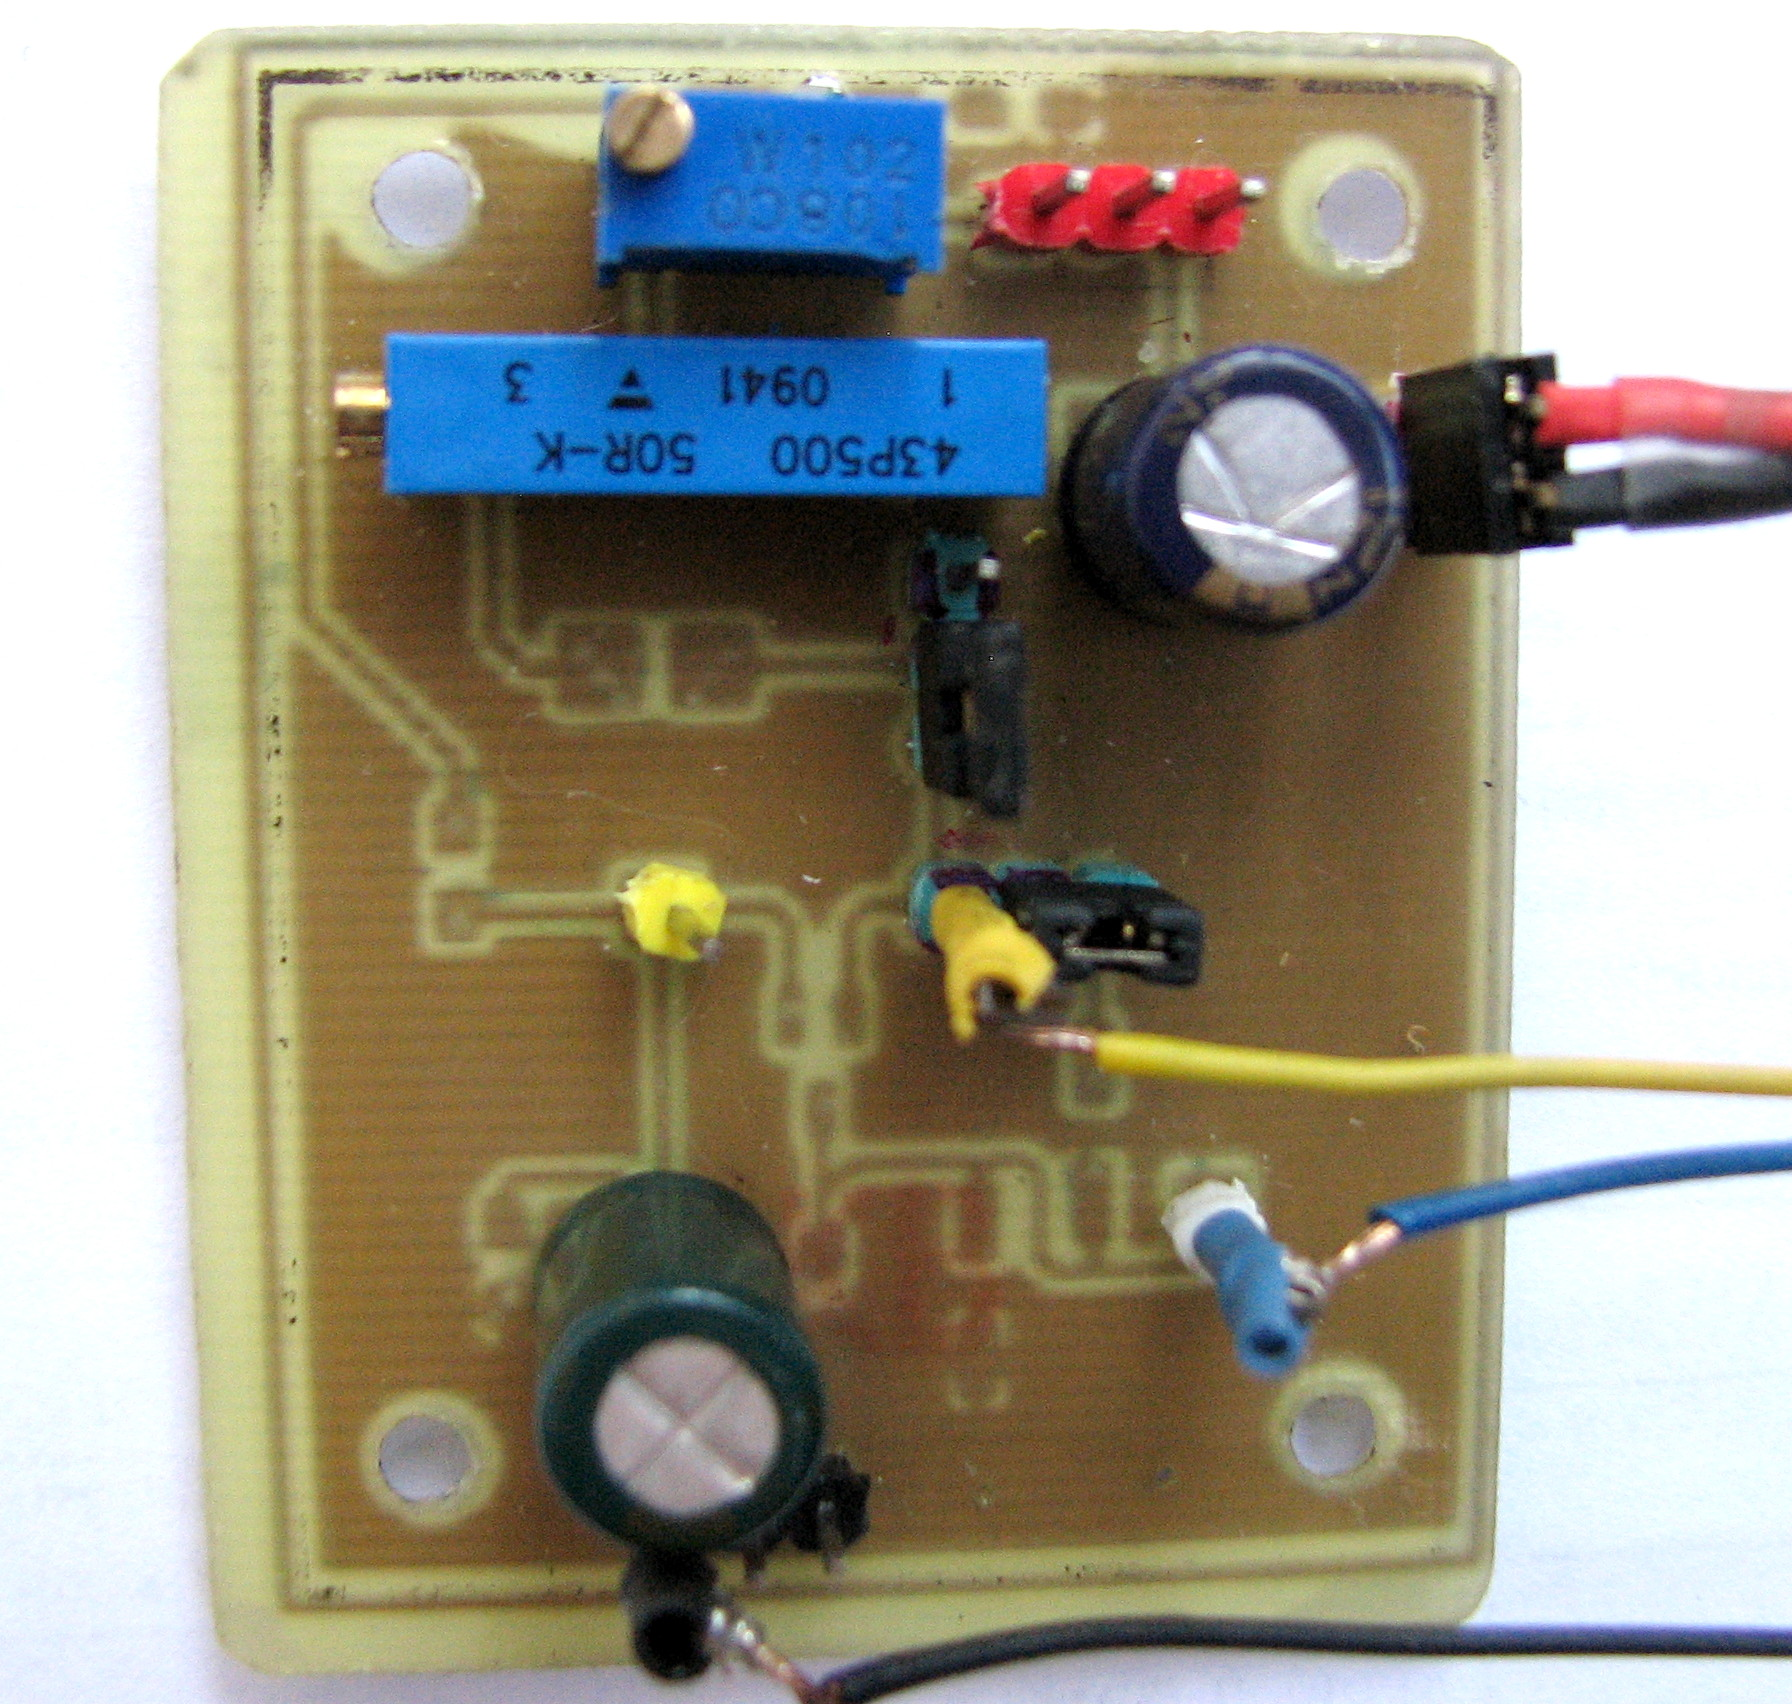
\includegraphics[width=0.5\textwidth]{p/colp_board.jpg} }
\caption{Друкована плата генератора Колпітца}
\label{atu:f:colp_board}
\end{figure}

Параметри всіх елементів, істотних для функціонування системи,
було виміряно до їх установки на друковану плату.

% }}}1


\section{Моделювання динаміки класичної моделі системи Колпітца і порівняння з реальним генератором}%{{{1

Для оцінки адекватності даної моделі були проведені
серії як обчислювальних, так і натурних фізичних
експериментів.
Моделювання проводилося в програмі ``qontrol''.
Для отримання даних з реального генератора був використаний
цифровий осцилограф Rigol DS1052E. З його допомогою були отримані
як візуальні уявлення аттракторов, так і оцифровані значення
сигналів
$V_e (t) $ і
$V_c (t) $. На попередньому етапі були визначені області простих
і складно-періодичних коливань, а також область чергування
хаотичних і складно-періодичних коливань.

При фізичному моделюванні, проведеному в рамках даної
роботи використовувалися наступні елементи з відповідними
параметрами:
%
\[
  V_{cc} = \SI{12.06}{\volt},          \;
  R_1 = R_2 = \SI{2.2}{\kilo\ohm},     \;
  R_e = \SI{430}{\ohm},
\]
%
\[
  C_1 = C_2 = \SI{1.03}{\micro\farad}, \;
  L = \SI{6.22}{\milli\henry},         \;
  T = \SI{305}{\kelvin},
\]
%
\[
  \text{Q: 2N2222A}, \quad
  h_{fe}=285, \;
  V_f = \SI{0.677}{\volt}, \;
  I_s = \SI{9.61e-14}{\ampere}, \;
  \alpha \approx 1.
\]

Тоді безрозмірні коефіцієнти приймають значення:
\[
 a = 77,     \quad
 c = 18.08,  \quad
 d = 0.19,   \quad
 e = 9.07.
\]
%
\[
F(z) =
\begin{cases}{l}
  e-1-z, & z \le e-1  \\
  0,     & z  >  e-1
\end{cases}.
\]

Діапазон зміни ідентифікованого параметра
$b \in [0.02; 4.2] $ визначається, з одного боку, власним опором котушки
індуктивності, з іншого --- зривом генерації.

На рис.~\ref{atu:f:colp_real_xzz}--\ref{atu:f:colp_model_f} представлені як
результати реального експерименту, так і дані, отримані в
результаті чисельного моделювання динаміки системи (\ref{atu:eq:colp}).
Представлені проекції аттракторов на площину
$(x + z, z) $ (природний вигляд для осцилографа), тривимірний вигляд
аттракторов, і спектри. На кожному малюнку представлено три
режими:звичайний, момент першого подвоєння періоду та хаотичний
режим.


\begin{figure}[htb!]
 \centerline{
   \includegraphics[width=0.32\textwidth]{p/mod/colp_m1_vv.png}
   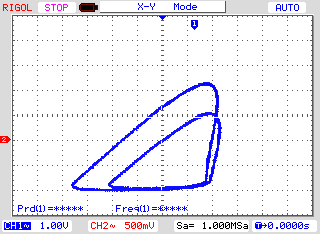
\includegraphics[width=0.32\textwidth]{p/mod/colp_m2_vv.png}
   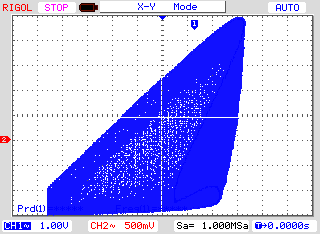
\includegraphics[width=0.32\textwidth]{p/mod/colp_m3_vv_ac.png}
 }
\caption{Проекції аттракторов реальної системи Колпітца на площину $ (x + z, z) $ для трьох режимів}
\label{atu:f:colp_real_xzz}
\end{figure}

Слід зазначити, що при проведенні вимірювань осцилограф зміг
визначити частоту коливань тільки для режиму простих коливань.


\begin{figure}[htb!]
 \centerline{
   \includegraphics[width=0.32\textwidth]{p/mod/colp_0-p_z_xpz_b=1x70.png}
   \includegraphics[width=0.32\textwidth]{p/mod/colp_0-p_z_xpz_b=1x37.png}
   \includegraphics[width=0.32\textwidth]{p/mod/colp_0-p_z_xpz_b=0x99.png}
 }
\caption{Проекції аттракторов моделі (\ref{atu:eq:colp}) системи Колпітца на площину $ (x + z, z) $ для трьох режимів}
\label{atu:f:colp_model_xzz}
\end{figure}



\begin{figure}[htb!]
 \centerline{
   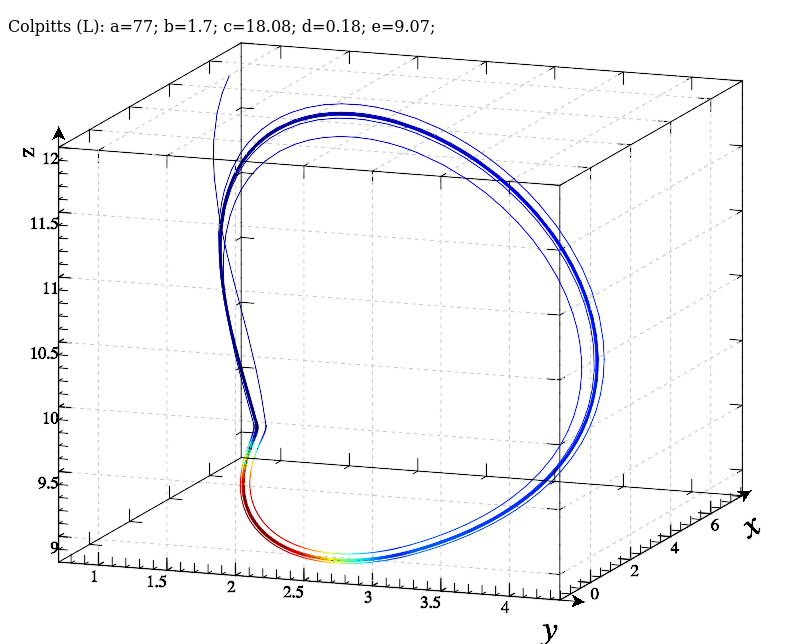
\includegraphics[width=0.32\textwidth]{p/mod/colp_0-p_xyz_b=1x70.png}
   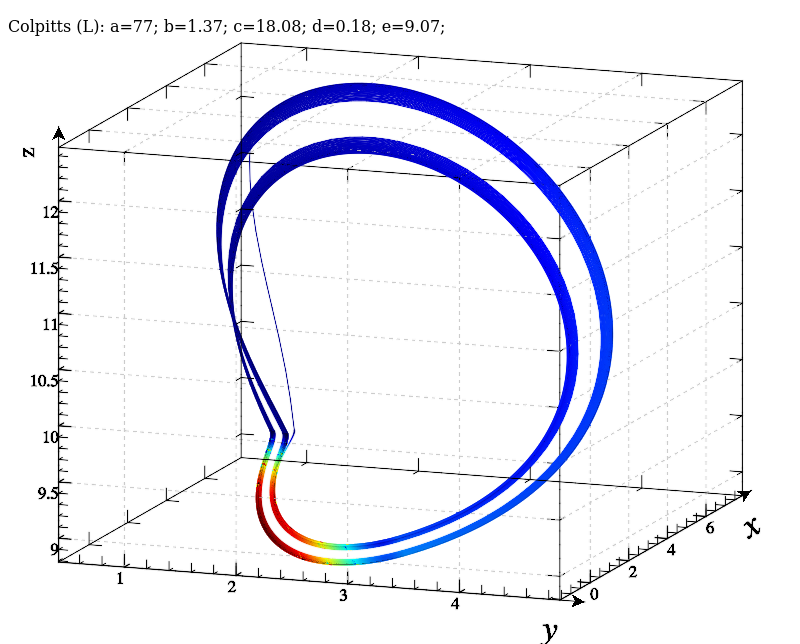
\includegraphics[width=0.32\textwidth]{p/mod/colp_0-p_xyz_b=1x37.png}
   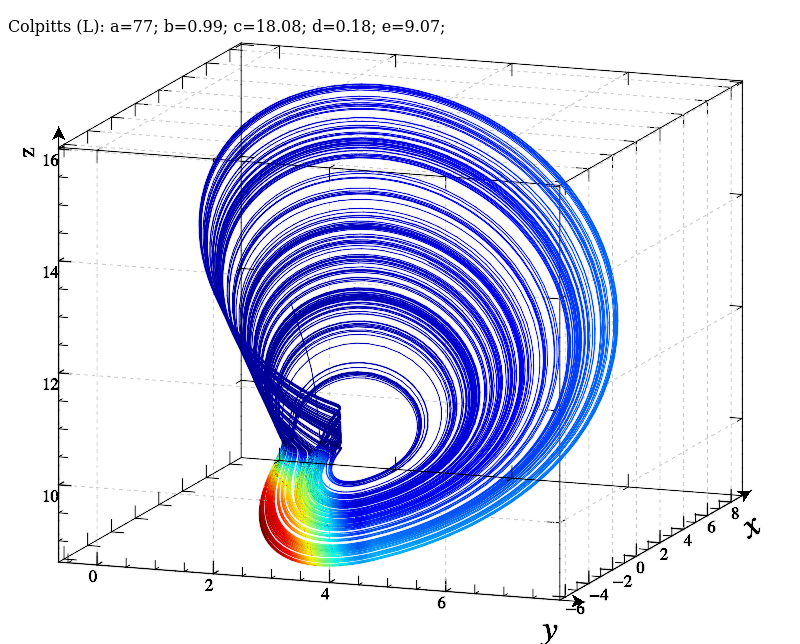
\includegraphics[width=0.32\textwidth]{p/mod/colp_0-p_xyz_b=0x99.png}
 }
  \caption{Аттрактори моделі (\ref{atu:eq:colp}) системи Колпітца для трьох режимів}
  \label{atu:f:colp_model_xyz}
\end{figure}

\begin{figure}[htb!]
 \centerline{
   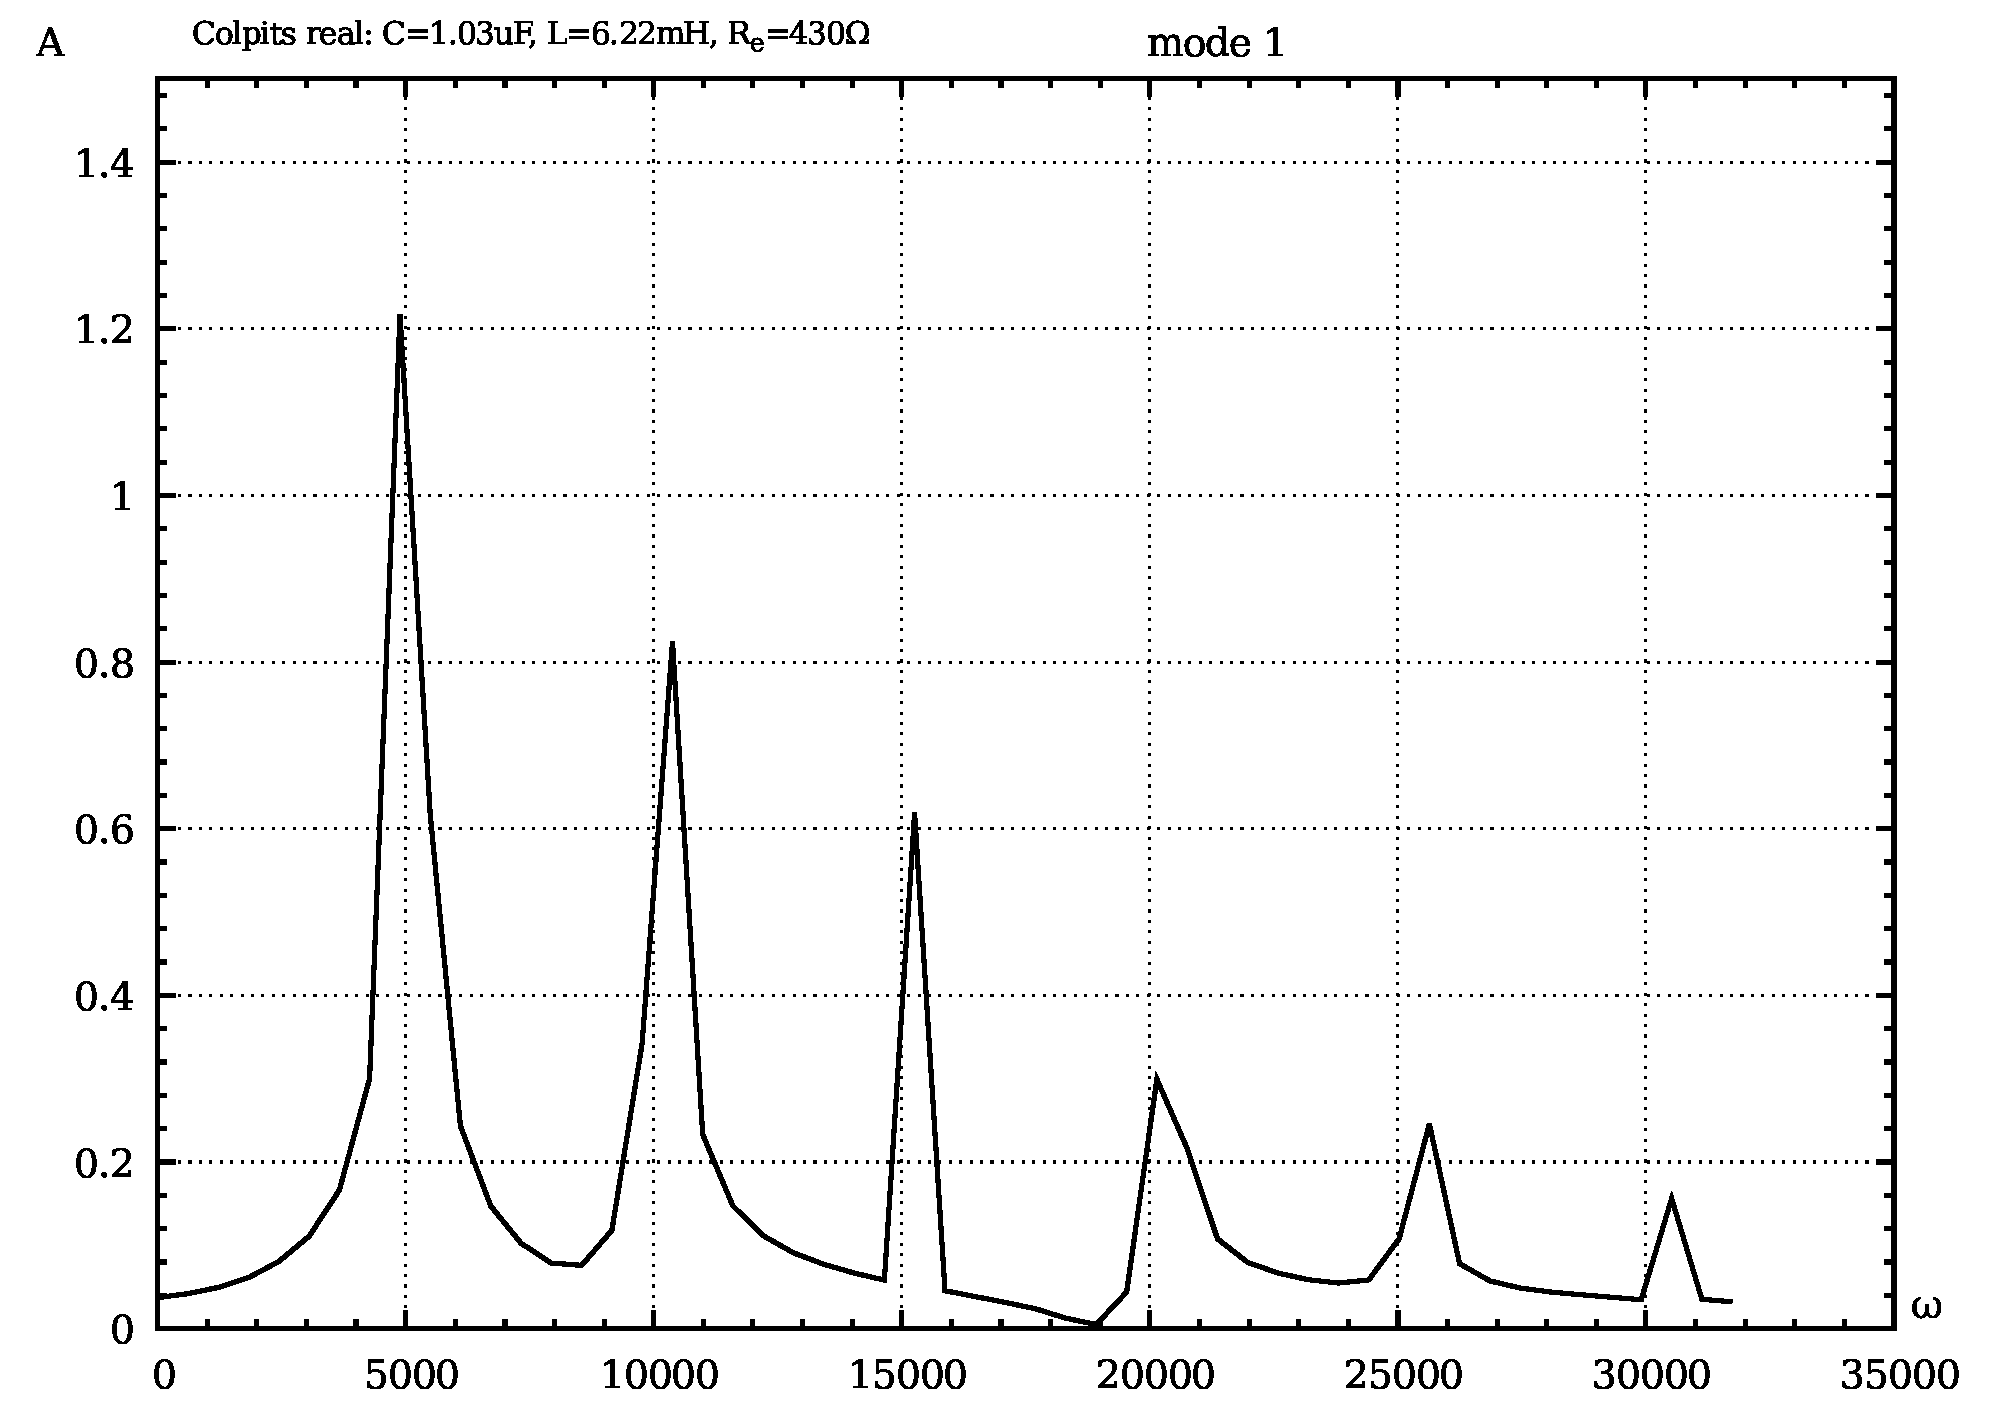
\includegraphics[width=0.32\textwidth]{p/mod/colp_m1_f.png}
   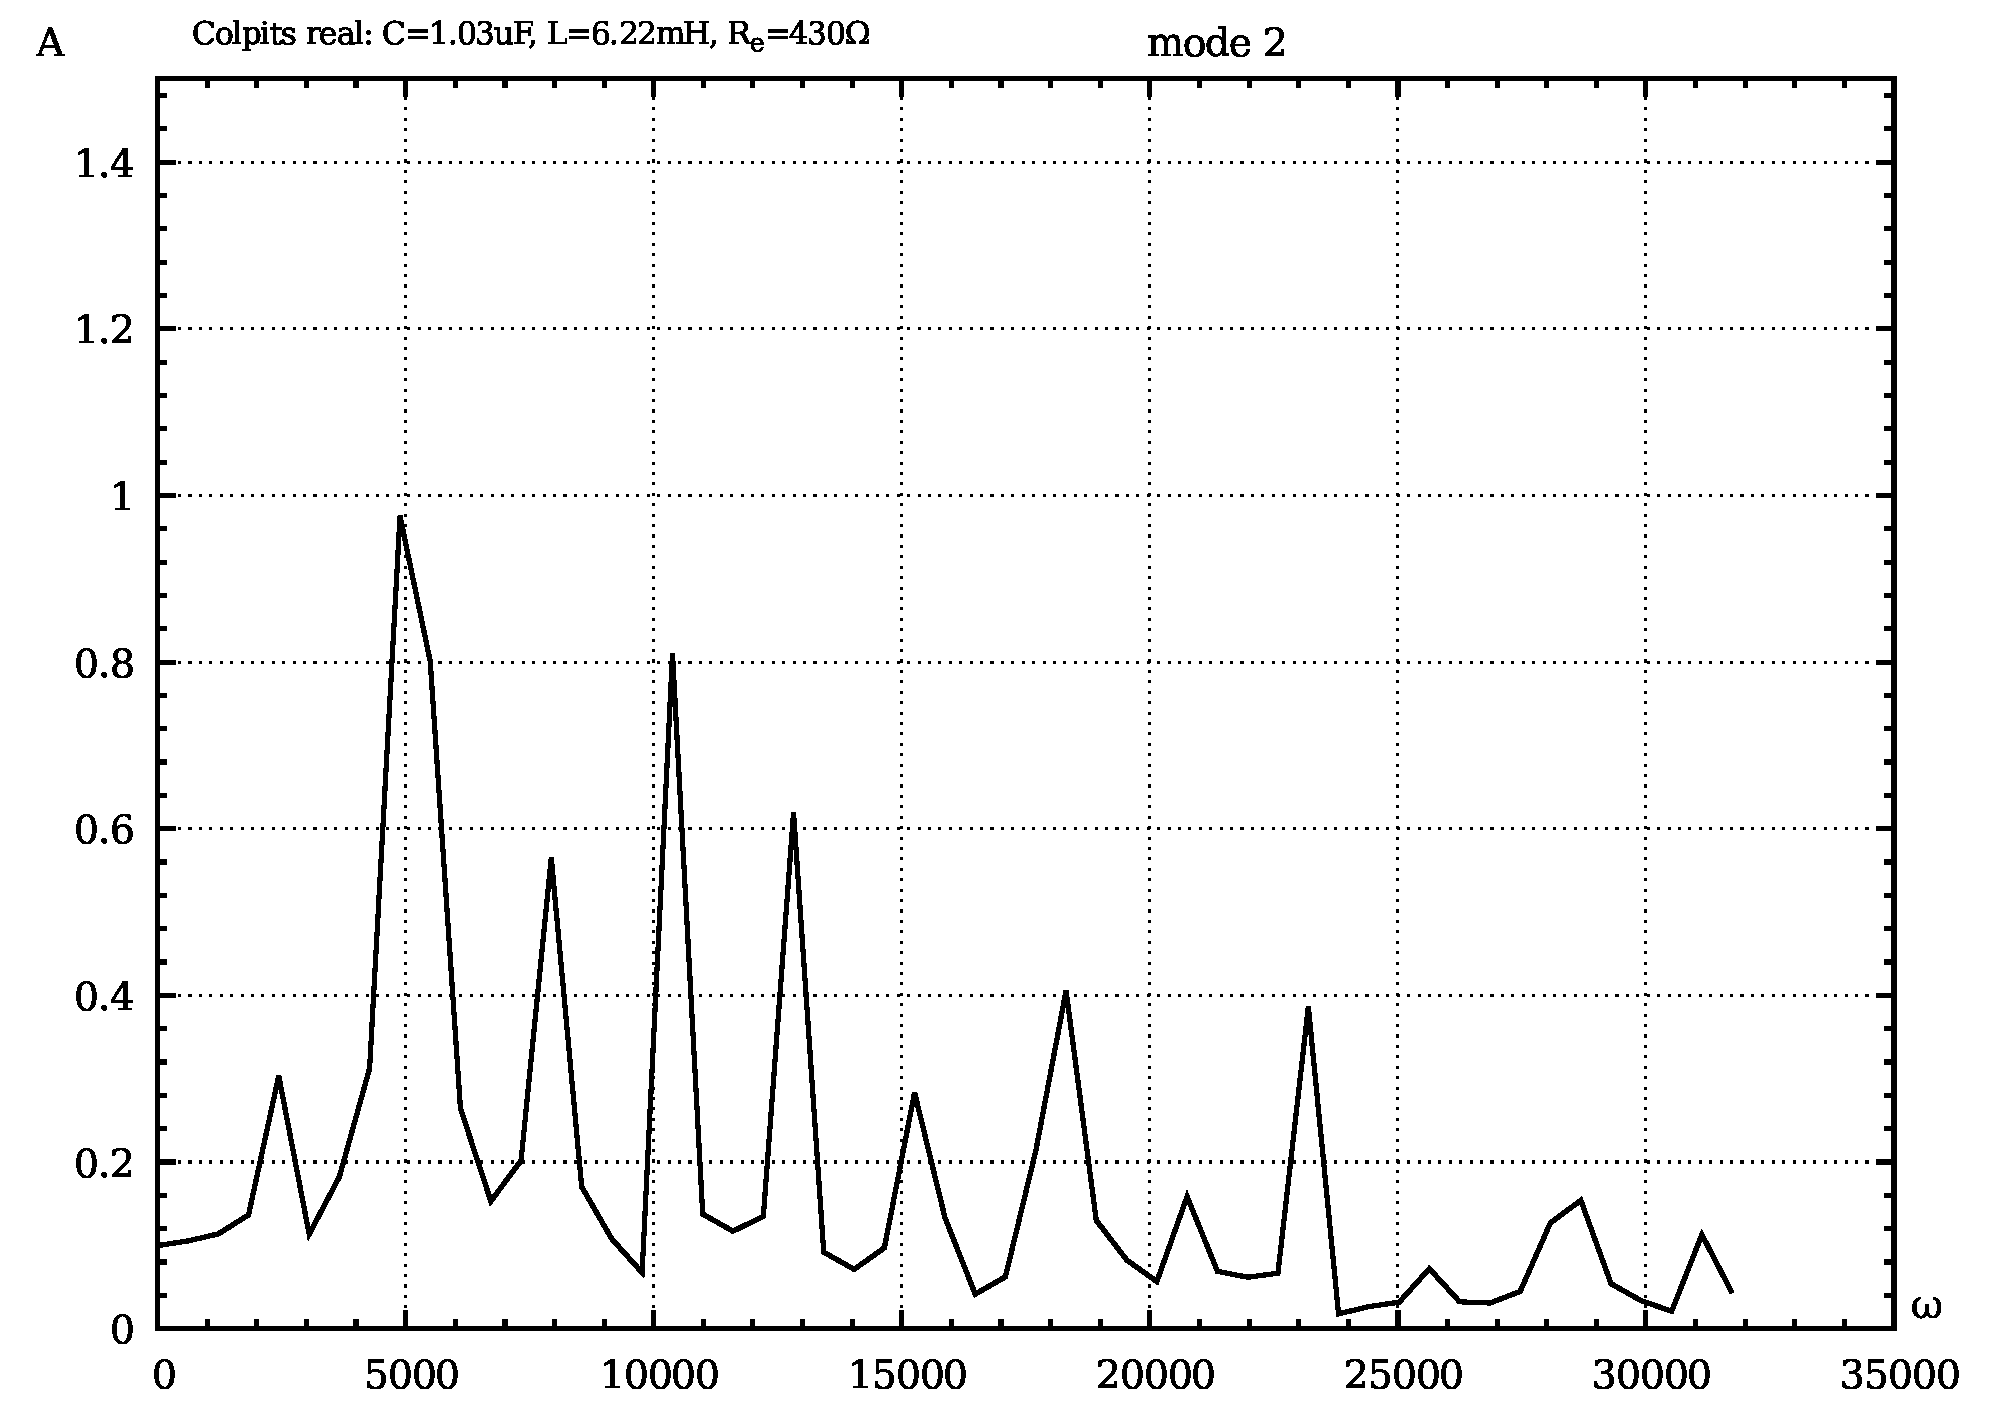
\includegraphics[width=0.32\textwidth]{p/mod/colp_m2_f.png}
   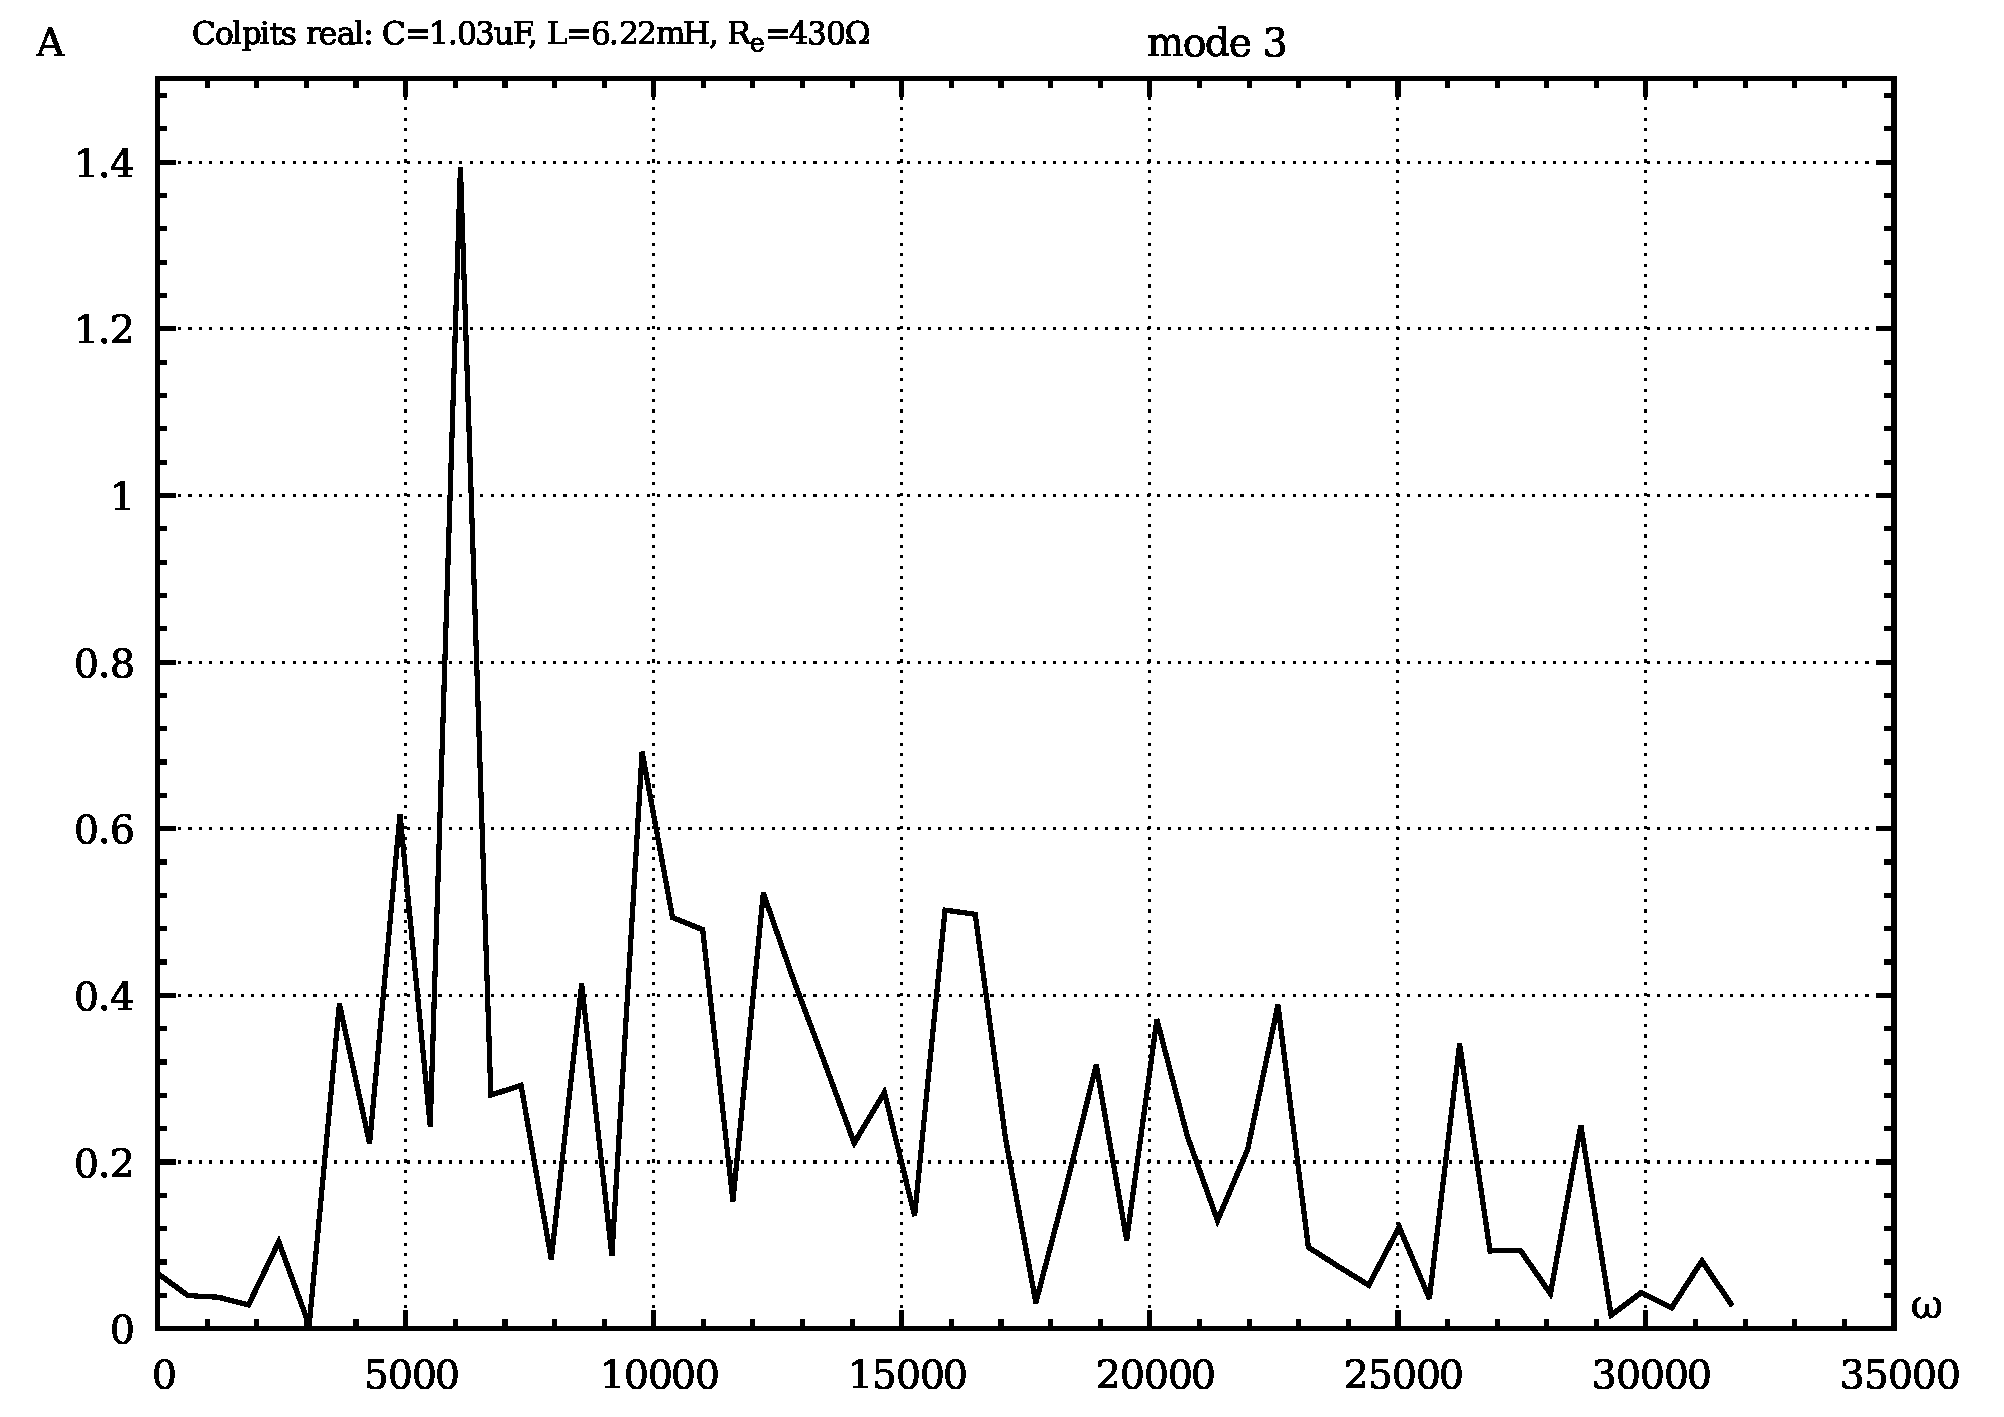
\includegraphics[width=0.32\textwidth]{p/mod/colp_m3_f.png}
 }
\caption{Спектри реальної системи Колпітца для трьох режимів}
\label{atu:f:colp_real_f}
\end{figure}

\begin{figure}[htb!]
 \centerline{
   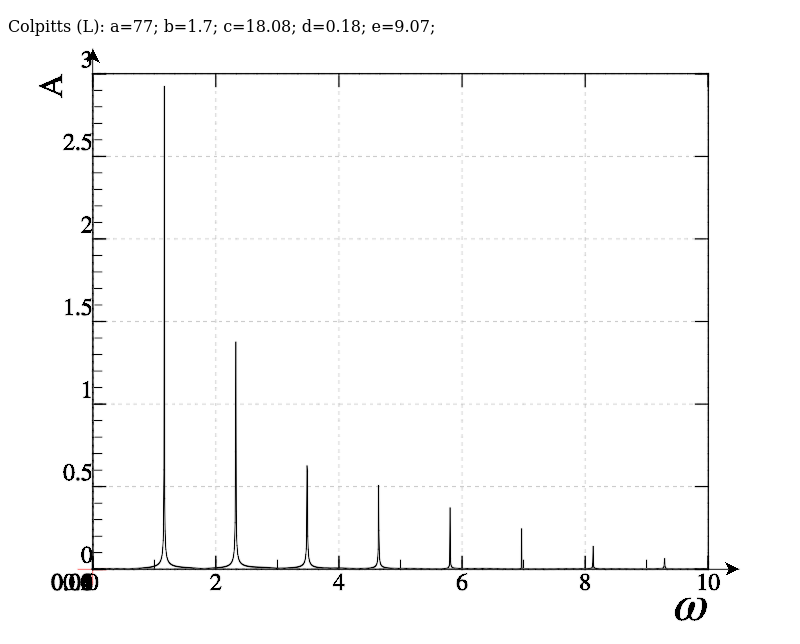
\includegraphics[width=0.32\textwidth]{p/mod/colp_f-p_f_b=1x70.png}
   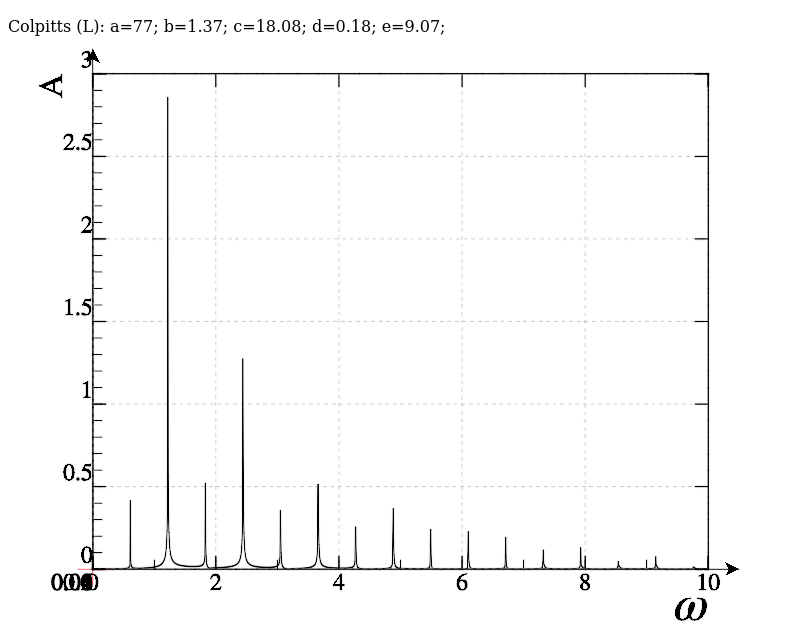
\includegraphics[width=0.32\textwidth]{p/mod/colp_f-p_f_b=1x37.png}
   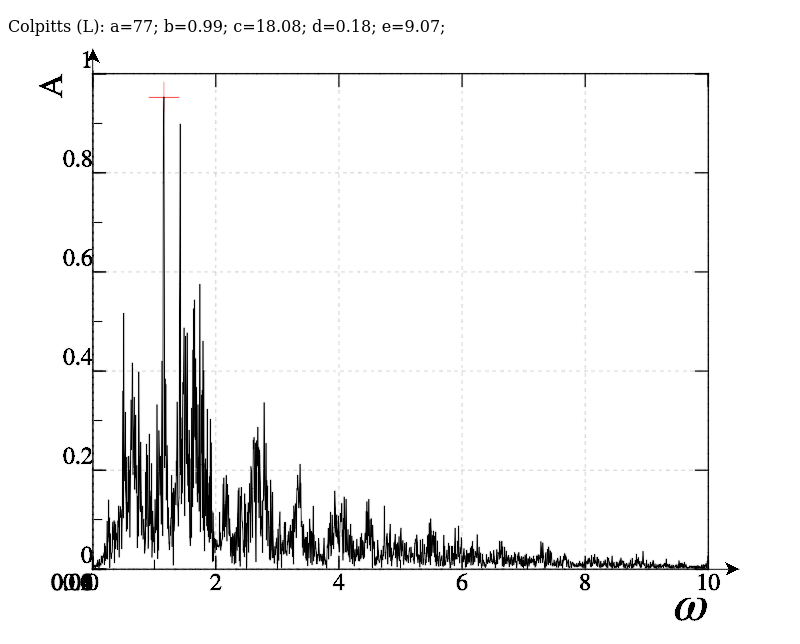
\includegraphics[width=0.32\textwidth]{p/mod/colp_f-p_f_b=0x99.png}
 }
\caption{Спектри моделі (\ref{atu:eq:colp}) системи Колпітца для трьох режимів}
\label{atu:f:colp_model_f}
\end{figure}


Порівняння результатів фізичного та чисельного моделювання
дозволяє зробити висновок про якісну схожість поведінки реальної
системи і моделі. Проте, величини параметра
$b $, при яких отримані розглядаються режими, збігаються тільки
приблизно. Для реальної системи значення параметра:
$b = 1.06, \; 0.94, \; 0.90 $, в той час як для моделі:
$b = 1.70, \; 1.34, \; 0.99 $. Розбіжність
значень, швидше за все, пов'язана з грубістю модельного уявлення
(\ref{atu:eq:bjt_libear_model}) транзистора. Питання застосовності різних
моделей біполярного транзистора в рамках даної системи вимагає
подальшого дослідження. З іншого боку, обмежений набір даних,
одержуваних з осцилографа (8192 відліку) не дозволяють отримати
досить докладний спектр реальної системи. Роздільна здатність у спектральної
області становила $\approx \SI{190}{\hertz} $.

% }}}1

\section{Критерії ідентифікації для класичної моделі системи Колпітца}%{{{1

Незважаючи на лише якісну подобу моделі (\ref{atu:eq:colp}) і реальної
системи, побудуємо систему ідентифікації з використанням
моделей даного виду. Це дозволить визначити можливість
ідентифікації для широко використовуваного в літературі
наближення.

Для визначення критерію ідентифікації розглянемо залежності
$q(b)$, отримані шляхом моделювання для системи Колпітца
(рис.~\ref{atu:f:colp_q}). При цьому слід врахувати, що найбільш просто
вимірюваними величинами є
$x$ і $z$, відповідні напругам
$V_1 $ і $ V_2 $. Перший набір залежностей дає два основні кандидати ---
$q_{x^2} $ і $ q_{z^2} $.
При цьому перший з них показує більш рівномірну
залежність. У той же час, більшість з розглянутих залежностей
мають явно виражений гіперболічний характер, особливо при
малих значеннях
$b $. Отже, в список кандидатів слід додати
$q_{x^{-2}} $ і $ q_{z^{-2}} $.

\begin{figure}[htb!]
\centerline{
  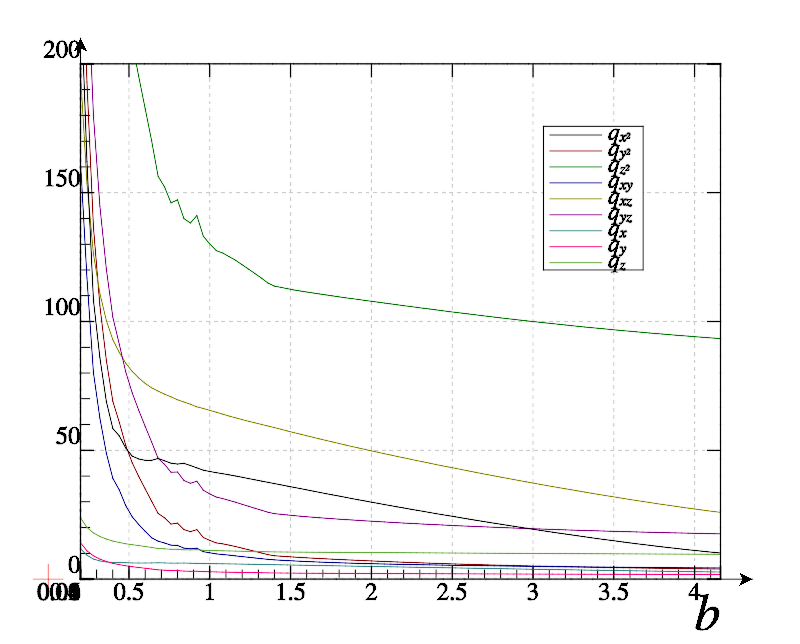
\includegraphics[width=0.49\textwidth]{p/mod/colp_p-p_b_e.png}
  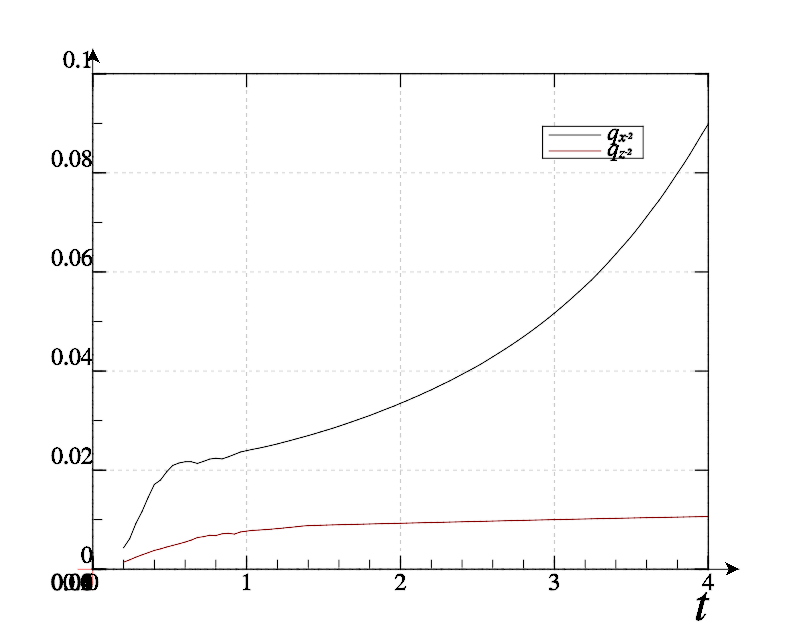
\includegraphics[width=0.49\textwidth]{p/mod/colp_p-p_b_1ex2.png}
}
  \caption{Залежності $q(b) $ для системи Колпітца (\ref{atu:eq:colp})}
\label{atu:f:colp_q}
\end{figure}

З графіків очевидно, що зворотні залежності не дають помітного
виграшу, тому виберемо величину
$q_{x^2} (b) $ як критерій.

% }}}1

\section{Моделювання процесів ідентифікації для класичної моделі генератора Колпітца} %{{{1

В якості системи ідентифікації була використана система з
п'ятьма пошуковими агентами і двома нерухомими моделями. Згідно
введеної класифікації, метод позначається як Fq3rlovngcF.$q_{x^2}$:5.
Аналогічно попереднім системам, для дослідження
динамічних властивостей системи ідентифікації залежності параметра
$b_o $ від часу були визначені як:
%
\begin{equation}
 b_o(t) = p_0 + U_p \sign \sin( \omega_p t ),
  \label{atu:eq:colp_b_sign}
\end{equation}
%
\begin{equation}
 b_o(t) = p_0 + U_p \sin( \omega_p t ).
  \label{atu:eq:colp_b_sin}
\end{equation}

Динаміка процесів ідентифікації для системи Колпітца
представлена на рис.~\ref{atu:f:colp_id}.

\begin{figure}[htb!]
  \PicDouble{p/mod/colp_m5p-pl_n_sign.png}{p/mod/colp_m5p-pl_n_sin.png}
\caption{Процес ідентифікації параметру $b$ системи (\ref{atu:eq:colp})
  за умов (\ref{atu:eq:colp_b_sign})~(a) і (\ref{atu:eq:colp_b_sin})~(b)
}
\label{atu:f:colp_id}
\end{figure}

Аналіз отриманих графіків дозволяє зробити висновок, що
система ідентифікації вийшла цілком працездатною. Звертає
на себе увагу зростання похибки ідентифікації при малих
значення параметра
$b$. Проте, з урахуванням тільки якісного подібності даної
моделі цим явищем цілком можна знехтувати.

% }}}1

\section{Вплив параметрів системи ідентифікації на похибку ідентифікації для класичної моделі системи Колпітца} %{{{1

Залежності
$\overline{e} (a_q) $ (рис.~\ref{atu:f:colp_e_a_q}) дозволяють коректно визначити час
усереднення. При цьому слід зазначити, що отримані результати
добре узгоджуються з спектрами системи.

\begin{figure}[htb!]
  \PicDouble{p/mod/colp_m5p-p_a_q_e_sign.png}{p/mod/colp_m5p-p_a_q_e_sin.png}
  \caption{Залежності  $\overline{e}(a_q)$ для системи (\ref{atu:eq:colp})
  за умов (\ref{atu:eq:colp_b_sign})~(a) і (\ref{atu:eq:colp_b_sin})~(b)
}
\label{atu:f:colp_e_a_q}
\end{figure}

Аналогічно, залежно середньоквадратичних похибок ідентифікації
від величини
$q_\gamma $ (рис.~\ref{atu:f:colp_e_qgamma}) дає інформацію про правильного
налаштування цього параметра системи ідентифікації.

\begin{figure}[htb!]
  \PicDouble{p/mod/colp_m5p-p_qg_e_sign.png}{p/mod/colp_m5p-p_qg_e_sin.png}
  \caption{Залежності  $\overline{e}(q_\gamma)$ для системи (\ref{atu:eq:colp})
  за умов (\ref{atu:eq:colp_b_sign})~(a) і (\ref{atu:eq:colp_b_sin})~(b)
}
\label{atu:f:colp_e_qgamma}
\end{figure}

Докладніший аналіз залежностей для даної системи практично
не має сенсу, зважаючи на обмеженість моделі.

% }}}1



\section{Уточнена модель генератора Колпітца} %{{{1

Як вже було зазначено, розглянута модель генератора Колпітца,
незважаючи на її широке використання при дослідженнях,
пов'язаних з хаотичною динамікою, має суттєві відмінності від
реального генератора. Переважна більшість елементів досить
добре описуються лінійним наближенням. Однак, є два елементи,
застосування лінійної моделі для яких або ж взагалі неможливо
(транзистор), або ж допустимо при певних умовах (індуктивність).

Як уже було згадано, більш точною моделлю транзистора є представлення
Еберса-Молла~\cite{horowitz}:
%
\begin{equation}
  I_c = I_s \left( \exp\frac{V_{be}}{U_t} - 1 \right),
  \label{atu:eq:ebers-moll}
\end{equation}
%
%\noindent
де
$I_s $ --- струм насичення (паспортна або отримана експериментально величина),
$U_t=kT/q$,
$q = \SI{1.6e-19}{\coulomb}$ --- заряд електрону,
$k = \SI{1.38e-23}{\joule/\kelvin}$ --
постійна Больцмана.
Необхідно врахувати, що в режимі відсічення ($ V_b <V_e $)
струм колектора дуже малий, а в режимі насичення
визначається іншими елементами схеми.

Існують і більш складні моделі, наприклад, модель
Гуммеля-Пуна~\cite{gummel_poon_1970,shiskin_electronnie_pribori} часто використовують
програми для моделювання електронних схем, наприклад ``Spice'' або ж її сучасні аналоги,
такі як ``ngspice''. У документації до
біполярним транзисторам прийнято вказувати їх характеристики
саме в термінах цієї моделі. У цій моделі враховують як значну
кількість нелінійних ефектів, так і явища, які відбуваються
при високих частотах.

При розробці фізичної реалізації генератора Колпітца його
параметри вибиралися так, що б змістити робочий діапазон
частот в область одиниць і десятків кілогерц. В першу чергу
це було зроблено з метою забезпечити працездатність наявних
і створених засобів вимірювання. При цьому, стає можливим
знехтувати високочастотними явищами, і тим самим, спростити
модель.

Сучасні біполярні транзистори характеризуються, як
правило, високим значенням параметра
$h_{fe}$. З урахуванням цього факту, а також особливості генератора
Колпітца, вираженої в підтримці постійного потенціалу бази,
можна знехтувати як струмом бази
$I_b$, так і відмінністю струму колектора
$I_c$ від струму емітера
$I_e$. При цьому, основним завданням моделювання транзистора як
частини генератора Колпітца є визначення
$I_c $, за умови, що задані значення потенціалів
$V_e $,
$V_c $ і
$V_b $. Тоді отримуємо:
%
\begin{equation}
  I_c
  = I_s \left( \exp\frac{V_{be}}{U_t N_f} - 1 \right)
    \cdot
    \left( 1 + \frac{V_{ce}}{V_{af}}\right),
  \label{atu:eq:bjt_model_sub}
\end{equation}
%
де
$N_f$ --- коефіцієнт неідеальності при прямому включенні,
$V_{af} $ --- напруга Ерлі в прямому включенні.

Після визначення
$I_c $ можна зробити один крок в чисельному рішенні рівняння
(\ref{atu:eq:colp_phys}). При цьому, перехід до безрозмірних величин в цій
постановці не дає помітних переваг, і не буде застосовуватися.

Як показала практика застосування чисельного рішення рівняння
(\ref{atu:eq:colp_phys}), безпосереднє застосування рівняння~(\ref{atu:eq:bjt_model_sub})
дуже легко призводить до обчислювальної нестійкості в режимі
насичення і близьких до нього. Це обумовлено експоненціальним ростом
$I_c $. Як правило, в цьому випадку застосовують зменшення кроку
за часом. Для набору використовуваних параметрів стійкість
розрахунків досягалася при кроці за часом близько
$\SI{1E-9}{\second} $, що робить процес розрахунку досить витратним.

З метою зменшити обчислювальні витрати при моделюванні, був
застосований наступний підхід. Після отримання значення
$I_c $, воно обмежувалося зверху величиною
$5 I_{c,\mathrm{st}}$,
де
$I_{c,\mathrm{st}} = \frac{V_{cc}}{R_{c,{\min}}+R_e}$ ---
максимальний струм через систему при відсутності коливань. Далі,
розраховувалася величина
%
\[
  R_{ce,\mathrm{eff}} = \frac{V_{ce}}{I_c} + R_{ce0},
\]
%
яка визначає ефективний опір транзистора з урахуванням омічного
опору переходів і контактів
$R_{ce0}$. Результуюче значення струму колектора визначалося так:
%
\[
  I_c = \frac{V_{ce}}{R_{ce,\mathrm{eff}}}.
\]

Цей підхід дозволив досягти стійкості моделювання при кроці
за часом близько
$\SI{5E-7}{\second} $ без помітного відмінності як від прямого
моделювання з дрібним кроком, так і від об'єкта. При подальшому
моделюванні був зроблений певний запас, і використовувався крок
$\SI{2E-7}{\second} $.

% Напруга Ерлі при прямому і інверсному включенні
%    double I_c0 = I_s * expm1( V_be / ( V_t * N_f ) )  * ( 1 + V_ce / V_af );
%    double R_ce = V_ce / I_c0 + R_ce0;

% }}}1


\section{Дослідження динаміки фізичної реалізації генератора Колпітца} %{{{1

Як уже зазначалося, використання в якості реєстратора даних
цифрового осцилографа класу Rigol DS1052E, незважаючи на гарну роздільну здатність
в часовій області ($ \SI{10}{\nano \second} $), швидкість і простоту отримання посвідки
аттрактора, має ряд істотних недоліків.

В першу чергу, за винятком режиму граничної частоти
дискретизації, немає можливості отримати досить довгу вибірку,
що сильно обмежує можливості спектрального аналізу. При аналізі
сигналів хаотичних і близьких до них систем особливо важливим
є спектральна роздільна здатність, яка визначається кількістю спостережень
при заданій частоті дискретизації. При недостатньої здатності
немає способу відрізнити ділянку суцільного спектра від
лінійного.

Також, обмежена розрядність вхідних АЦП (8 біт) призводить до
відносно високого рівня шумів квантування. При цьому, наявність
тільки двох каналів вимірювання не дозволяє отримати вид
аттрактора для системи з трьома координатами.

Для усунення цих недоліків був створений вимірювальний
комплекс на основі мікроконтролера STM32F746. У якості ядра системи було використано
плату Waveshare STM32F746. Крім власне контролера, на ній
встановлена пам'ять SDRAM 8MB, що дозволило зберігати
в сумі до 4 мільйонів відліків. Використовувалося до чотирьох
каналів 12-ти АЦП з роздільною здатністю 12~біт. Використання
зовнішніх АЦП з більшою розрядністю~\cite{atu_st104a} для даного
завдання видається дещо надмірним. З урахуванням обмеження
$2 \cdot 10 ^ 6 $ відліків в секунду (з використанням DMA для пересилання
отриманих даних в пам'ять і таймера як сигналу для початку
вимірювань), максимальна досяжна частота дискретизації в цих
умовах досягає
$\SI{500}{\kilo \hertz} $, що для досліджуваної системи надлишкове,
але дозволяє переконатися у тому, що не була втрачена частина
спектру.

Для управління мікроконтролером була створена програма на
мові C++. Так як для даного вимірювання потрібно як квазі-одночасне,
так і повністю одночасне виконання різних дій, то була
використана мініатюрна операційна система реального часу для
мікроконтролерів FreeRTOS. Управління програмою здійснювалося
в режимі терміналу з використання протоколу UART. Реалізована
в програмі система команд дозволяє налаштовувати параметри
вимірювання, проводити саме вимірювання, і зберігати результат.

В якості основного способу збереження результату
використовувалася SDHC карта, підключена по протоколу SDIO з однією
лінією даних. Слід зазначити, що при проведенні вимірювання
обов'язковою умовою є відключення SDIO підсистеми контролера. В
іншому випадку рівень шумів вимірювання не дозволяє отримати
значущі результати. Альтернативним способом збереження
даних є використання того ж каналу, який використовується для
передачі команд і прийому відповіді на них --- UART. Для збереження
результатів в файл застосовуються засоби використовуваної
програми емуляції терміналу. Однак, відносно низька швидкість
такого способу передачі даних вимагає тривалого часу для
збереження результатів.

Важливою умовою отримання даних є узгодження рівнів сигналів
в досліджуваній системі з допустимими вхідними рівнями
АЦП. Амплітудне значення сигналів в даній системі досягало
$\SI{15}{\volt} $, в той час як вхідна напруга АЦП не повинно
перевищувати
$\SI{3}{\volt} $. Використання для узгодження резистивного дільника
для даної схеми не виправдано. Малий повний опір подільника
спотворює динаміку досліджуваної системи, особливо в умовах
хаотичних коливань. Вищі значення призводять до зростання шумів
вимірювання і неможливості використання захисних засобів,
наприклад, пар діодів для захисту вхідних ланцюгів контролера.

Тому, для узгодження використовувалася мікросхема TL074, що
об'єднує в одному корпусі 4 операційних підсилювача, які
характеризуються високим вхідним опором ($ \approx \SI{1e12}{\ohm} $),
низьким рівнем нелінійних спотворень ($ \approx 0.003 \% $),
відповідним для даного завдання частотним
діапазоном і допустимими вхідними напругами. Кожен з
підсилювачів включався в режимі повторювача~\cite{horowitz}, і на
його вихід був підключений резистивний дільник з підібраними
опорами і два захисних діода.

Перед кожною серією експериментів проводилося калібрування
вимірювального комплексу на набір заданих значень напруг. Після
вимірювань проводилася перевірка на стабільність параметрів,
і в разі негативного результату дані відкидалися.


У першій серії експериментів значення параметра
$R_c $ було для кожного експерименту фіксованим, та було встановлено
перед кожним експериментом. Використовувався нерівномірний
ряд значень параметра в діапазоні
$[25.3; 100] \SI{}{\ohm} $. У тих областях, де спостерігалася складна
поведінка, відстань між точками була меншою.

Система реєстрації даних працювала з використанням чотирьох
каналів вимірювання. Вимірювалися сигнали:
$V_e(t) = V_1(t)$,
$V_c(t) = V_1(t) + V_2(t)$,
$V_{ca}(t)$ ---
потенціал на контакті 1 роз'єму $ \mathrm{P}_3 $,
$V_cc(t)$.
Сигнал
$V_2 (t) $ визначався як
$V_c (t) - V_e (t) $. Струм через котушку індуктивності оцінювався як
$I_L = \frac{V_{cc} (t) - V_{ca} (t)}{R_{cv1} + R_{cv2}} $. Сигнал
$V_{cc} (t) $ використовувався для контролю калібрування системи
реєстрації, а також для перевірки відсутності пульсацій напруги
живлення.



При відносно високих значення параметра
$R_c $ спостерігається регулярна динаміка і лінійчатий
спектр~(рис.~\ref{atu:f:colp_r_attr_f_50}).

\begin{figure}[htb!]
  \PicDouble{p/r/v1iv2_050000.png}{p/r/f_050000.png}
  \caption{Аттрактор~(a) і спектр~(b) реального генератора Колпітца при $ R_c = \SI{50}{\ohm} $}
\label{atu:f:colp_r_attr_f_50}
\end{figure}

При зменшенні значення
$R_c $ відбувається подвоєння періоду, що відображається у вигляді
другої петлі аттрактора і появою приблизно вдвічі менших частот
в спектрі~(рис.~\ref{atu:f:colp_r_attr_f_40}).

\begin{figure}[htb!]
  \PicDouble{p/r/v1iv2_040000.png}{p/r/f_040000.png}
  \caption{Аттрактор~(a) і спектр~(b) реального генератора Колпітца при $ R_c = \SI{40}{\ohm} $}
\label{atu:f:colp_r_attr_f_40}
\end{figure}

Подальше зменшення значення параметра, через каскад біфуркацій,
призводить до появи дивного аттрактора і суцільного спектра
(рис.~\ref{atu:f:colp_r_attr_f_30}).

\begin{figure}[htb!]
  \PicDouble{p/r/v1iv2_030000.png}{p/r/f_030000.png}
  \caption{Аттрактор~(a) і спектр~(b) реального генератора Колпітца при $ R_c = \SI{30}{\ohm} $}
\label{atu:f:colp_r_attr_f_30}
\end{figure}

При цьому, на відміну від системи Лоренца, при подальшій
зміні параметра відбувається чергування хаотичного і
складно-періодичного режимів (рис.~\ref{atu:f:colp_r_attr_f_29}).

\begin{figure}[htb!]
  \PicDouble{p/r/v1iv2_029000.png}{p/r/f_029000.png}
  \caption{Аттрактор~(a) і спектр~(b) реального генератора Колпітца при $ R_c = \SI{29}{\ohm} $}
\label{atu:f:colp_r_attr_f_29}
\end{figure}

На відміну від системи збору даних, що була заснована на цифровому
осцилографі, роздільна здатність в спектральної області склала
$\SI{1}{\hertz} $, що дозволило впевнено відрізняти спектри хаотичної
і складно-періодичної динаміки.

% }}}1

\section{Аналіз і вибір критеріїв}  % {{{1

При ідентифікації класичної моделі генератора Колпітца був
використаний критерій
$q_{x^2} $. Заміна моделі на нову вимагає провести аналіз критеріїв
повторно. На рис.~\ref{atu:f:colp_bjt_q-p_Rc_q} представлені залежності
досліджуваних критеріїв від значення
$R_c $, для нової моделі.

\begin{figure}[htb!]
\centerline{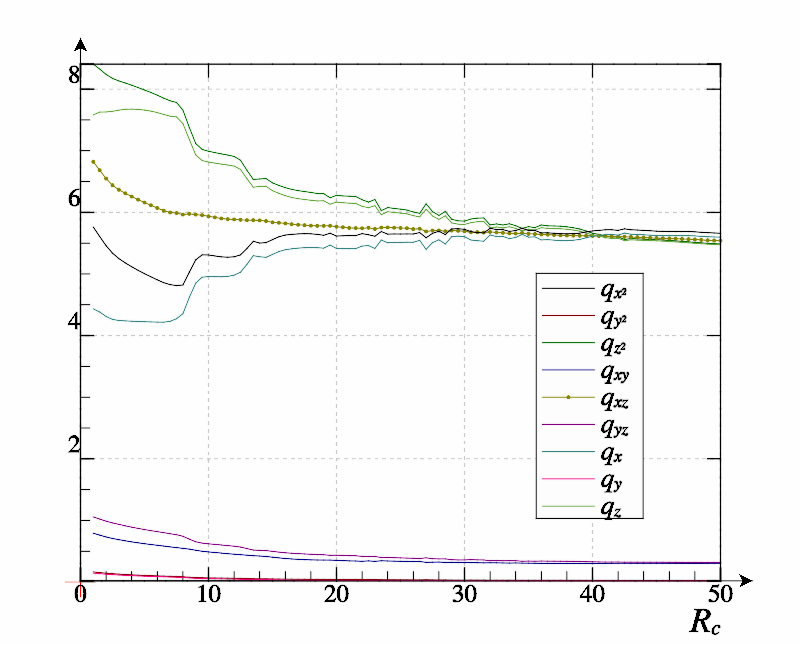
\includegraphics[width=0.7\textwidth]{p/colp_bjt_q-p_Rc_q.png} }
\caption{Залежності значень критеріїв ідентифікації для моделі системи Колпітца}
\label{atu:f:colp_bjt_q-p_Rc_q}
\end{figure}

Істотне порушення монотонності як для раніше використовуваного
критерію
$q_{x^2} $, так і для іншого кандидата ---
$q_{z^2} $, особливо в областях, де спостерігається хаотична
динаміка, не сприяє успішному процесу ідентифікації. З іншого
боку, критерій
$q_{xz} $ проявляє монотонну залежність, принаймні для моделі.

Розглянемо залежності цих же критеріїв, але для реального
генератора, отримані на підставі даних з попередньої серії
експериментів з фіксованим значенням параметра. Отримані
залежності представлені на рис.~\ref{atu:f:colp_read_q-p_Rc_q-p_Rc_q}.


\begin{figure}[htb!]
\centerline{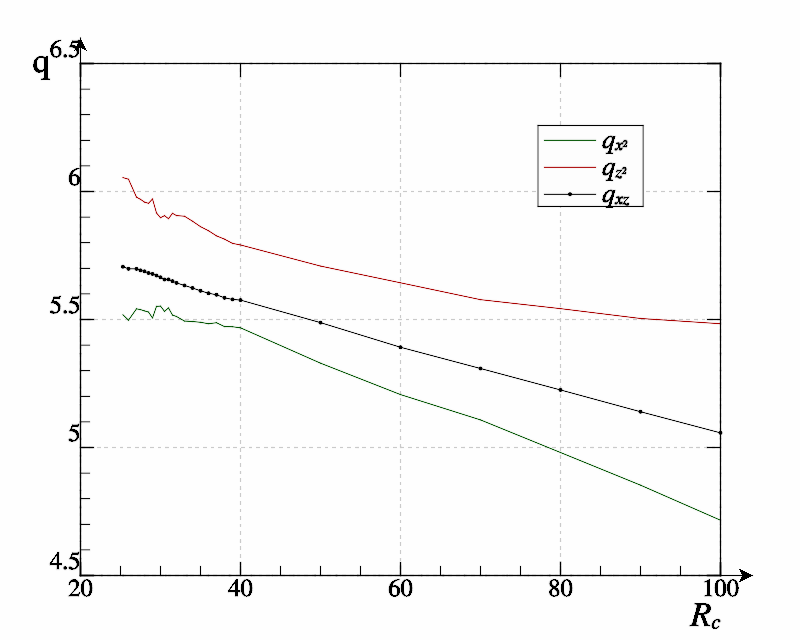
\includegraphics[width=0.7\textwidth]{p/colp_read_q-p_Rc_q.png} }
\caption{Залежності значень критеріїв ідентифікації $q_{x^2}$, $q_{z^2}$ і $q_{xz} $ для реального генератора Колпітца}
\label{atu:f:colp_read_q-p_Rc_q-p_Rc_q}
\end{figure}

Для реального генератора спостерігається картина, яка практично
збігається з результатами, отриманими для моделі. Таким чином,
критерій $q_{xz}$ потенційно є найкращим серед розглянутих.

Для успішної ідентифікації необхідна не тільки схожість
залежностей критерію від параметра для моделі і об'єкта, а й
близькість їх значень. На рис.~\ref{atu:f:colp_q_cml} наведено залежності
$q_{xz}(R_c)$ як для об'єкта, так і для моделі.

\begin{figure}[htb!]
\centerline{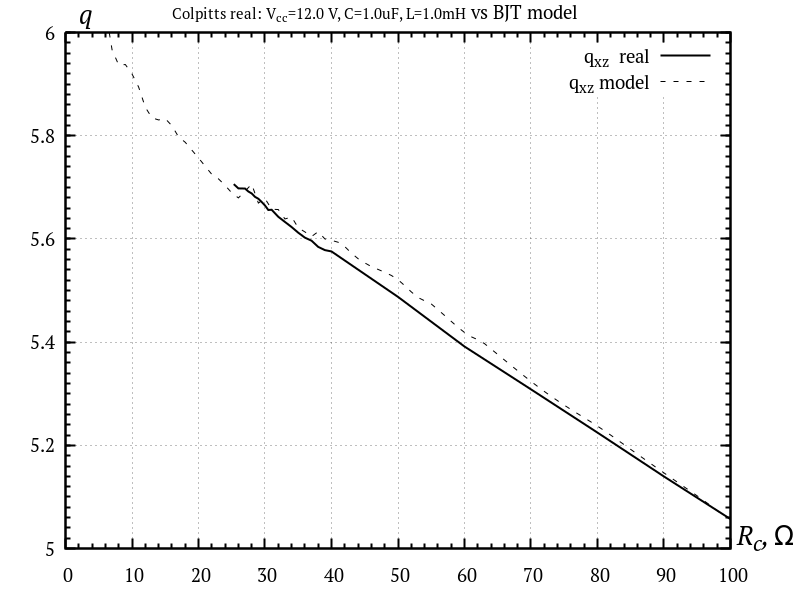
\includegraphics[width=0.7\textwidth]{p/colp_q_cml.png} }
\caption{Порівняння залежностей значень критерію ідентифікації $ q_{xz} $ реального генератора Колпітца з моделлю}
\label{atu:f:colp_q_cml}
\end{figure}

Спостерігається хороший рівень збігу, що свідчить не тільки
про правильність вибору критерію, а й про адекватність нової
моделі в цілому. Графік залежності для реального об'єкта має
меншу область визначення, що пов'язано з фізичними обмеженнями
конкретного об'єкта.

Незважаючи на достатню для працездатності ідентифікації
близькість графіків, слід зазначити і певні недоліки даного
критерію. Перш за все, спостерігається практично однакова
відстань між графіками при
$R_c> \SI{40}{\ohm} $, тобто в тих областях, де спостерігається регулярна
динаміка. На підставі наявних даних немає можливості визначити,
чим конкретно викликана ця розбіжність, однак, слід припускати
помітну статичну похибку ідентифікації в цій області. Також, в
межах робочої області значення критерію змінюється слабо. Як
наслідок, очікується підвищена чутливість ідентифікації до
перешкод при вимірюванні.

% }}}1

\section{Синтез і аналіз системи ідентифікації} %{{{1


Для перевірки працездатності системи ідентифікації в умовах
нестаціонарного параметра, а також для аналізу характеристик
цієї системи, необхідно забезпечити контрольовану зміну
значення параметра. Становище ускладнюється тим, що необхідні
значення зміни опору досить малі, порядку одиниць і десятків
Ом, що виключає застосування цифрових потенціометрів. Для
реалізації можливості змінювати значення параметра були
зроблені наступні кроки. До роз'єму
$\mathrm{P}_3 $ була підключена додаткова схема з незалежним
живленням, що складається з послідовно включених змінного
резистора і MOSFET транзистора логічного рівня з малим опором у
відкритому стані. Значення опору змінного резистора в кожному
експерименті підбиралось таки чином, щоб його опір з урахуванням
паралельного включення з резисторами
$R_{cv1} $ і
$R_{cv2} $ забезпечувало необхідне значення меншого опору, а тільки
$R_{cv1} + R_{cv2 } $ --- більшого.

Для керування включенням MOSFET транзистора використовувалося
два підходи. У першому транзистором керував окремий генератор
на таймері 555. Цей підхід досить простий в реалізації, однак
його застосування ускладнює завдання синхронізації при
визначенні похибки ідентифікації. Тому кращим виявився
другий підхід, при якому включенням керував сам контролер
через оптичну розв'язку. Таким чином, перемикання відбувалися
в задані моменти часу, прив'язані до моменту запуску АЦП,
що значно спрощує аналіз помилок ідентифікації. Загальний
вигляд установки для проведення ідентифікації призведе на
рис.~\ref{atu:f:colp_r_id_dev}. Частина елементів, наприклад SDHC накопичувач,
знаходиться під іншими частинами установки.


\begin{figure}[htb!]
  \centerline{
    \includegraphics[width=0.80\textwidth]{p/colp_stand.png}
  }
\caption{Загальний вигляд установки для ідентифікації нестаціонарного параметра $ R_c $ реального генератора Колпітца}
\label{atu:f:colp_r_id_dev}
\end{figure}

Природним недоліком такого підходу є те, що так можна
забезпечити тільки стрибкоподібну динаміку зміни
параметра. Однак, це не є принциповим недоліком, тому що якщо
система ідентифікації є працездатною в таких умовах, то вона
збереже працездатність і в разі плавної зміни параметра.

Для процесів параметричної ідентифікації генератора Колпітца
представлені результати чотирьох експериментів, проведених в
схожих умовах. Використовувалася група методів ідентифікації
``ql3rlWvnAAW''.

% C_1, C_2 = 1.0 uF, L = 1.0 mH, R_l=24.2 Ohm, R_e = 300 Ohm, R_1 = R_2 = 2.0 kOhm,
% Q: MMBT2222A: h_{FE}=210, V_{je} = 0.667V.
% V_{cc} = 12.0 V, V_{b} = 5.94 V
% d_0.txt: 27.0 - 50.0 Ohm  28.5  +-  11.5
% d_1.txt: 29.5 - 35.0 Ohm  32.25 +-  2.75
% d_2.txt: 32.0 - 40.0 Ohm  36.0  +-  4.0
% d_3.txt: 28.0 - 37.0 Ohm  32.5  +-  4.5
% old:
% d_0.txt: 27.3 - 44.2 Ohm  35.75 +-  8.45
% d_1.txt: 29.0 - 35.0 Ohm  32    +-  3
% d_2.txt: 26.0 - 30.0 Ohm  28    +-  2
% d_3.txt: 31.0 - 52.0 Ohm  41.5  +- 10.5
% d_4.txt: 29.0 - 32.0 Ohm  30.5  +-  1.5

Параметри першого експерименту для генератора Колпітца
%
\begin{equation}
  \begin{array}{c}
    R_{c,\min} = \SI{27.0}{\ohm};
    \;
    R_{c,\max} = \SI{50.0}{\ohm};
    \;
    T_{R_c} = \SI{200}{\milli\second};
  \\
    R_c(t) = \SI{28.5}{\ohm} + \SI{11.5}{\ohm} \cdot \sign \sin \left(  \frac{\pi t}{T_{R_c}}  \right)
  \end{array}
  \label{atu:eq:colp_test1_cond}
\end{equation}
%
були підібрані таки чином, що б зміна значення параметра
приводила до переходу від хаотичного режиму до періодичного.

Як видно з графіків, що відображають процес
ідентифікації~(рис.~\ref{atu:f:colp_r_id_1}), система ідентифікації
виявилася цілком працездатною.


\begin{figure}[htb!]
  \PicDouble{p/r/colp_real_id-p_t_pi_ql3rlWvnAAW_real_d_0.png}{p/r/colp_real_id-p_t_p_ql3rlWvnAAW_real_d_0.png}
  \caption{Процес ідентифікації параметра $ R_c $ реального генератора Колпітца за умов (\ref{atu:eq:colp_test1_cond}): динаміка агентів~(a) та $p_\mathrm{id}$~(b)}
  \label{atu:f:colp_r_id_1}
\end{figure}


При цьому слід зазначити значну похибку ідентифікації при
$R_c = \SI{50}{\ohm} $. Її появу слід було очікувати, ураховуючи вже
згадану різницю в значеннях критерію для об'єкта і моделі. При
цьому спостерігається досить рідкісне явище --- одну з найменших
помилок ідентифікації показав метод координатора пошуку
$p_{gc} $. Це пов'язано з тим, що цей метод характеризується
зміщенням ідентифікованого значення до центру робочої області в
випадках, коли це значення знаходиться
поблизу краю цій області. Таким чином, одна похибка компенсувала
іншу. Однак, це досить рідкісний окремий випадок, і не варто
розглядати отриманий результат як перевагу методу
$p_{gc}$.


Параметри другого експерименту для генератора Колпітца
%
\begin{equation}
  \begin{array}{c}
    R_{c,\min} = \SI{29.5}{\ohm};
    \;
    R_{c,\max} = \SI{35.0}{\ohm};
    \;
    T_{R_c} = \SI{200}{\milli\second};
  \\
    R_c(t) = \SI{32.25}{\ohm} + \SI{2.75}{\ohm} \cdot \sign \sin \left( \frac{\pi t}{T_{R_c}}  \right)
  \end{array}
  \label{atu:eq:colp_test2_cond}
\end{equation}
%
відповідають перемиканням динаміки системи між хаотичним і
складно-періодичним режимами.

Результати моделювання процесів ідентифікації, представлені
на рис.~\ref{atu:f:colp_r_id_2}, відображають не тільки збереження
працездатності, але і зменшення похибки ідентифікації через
роботу на тій ділянці критерію, на якому відмінність між об'єктом
і моделлю мінімально.

\begin{figure}[htb!]
  \PicDouble{p/r/colp_real_id-p_t_pi_ql3rlWvnAAW_real_d_1.png}{p/r/colp_real_id-p_t_p_ql3rlWvnAAW_real_d_1.png}
  \caption{Процес ідентифікації параметра $ R_c $ реального генератора Колпітца за умов (\ref{atu:eq:colp_test2_cond}): динаміка агентів~(a) та $p_\mathrm{id}$~(b)}
\label{atu:f:colp_r_id_2}
\end{figure}


Параметри третього експерименту для генератора Колпітца
%
\begin{equation}
  \begin{array}{c}
    R_{c,\min} = \SI{32.0}{\ohm};
    \;
    R_{c,\max} = \SI{40.0}{\ohm};
    \;
    T_{R_c} = \SI{200}{\milli\second};
  \\
    R_c(t) = \SI{36.0}{\ohm} + \SI{4.0}{\ohm} \cdot \sign \sin \left(   \frac{\pi t}{T_{R_c}}   \right)
  \end{array}
  \label{atu:eq:colp_test3_cond}
\end{equation}
%
відповідають переходу між двома складно-періодичними режимами
з різною кількістю петель в аттракторі.

При цьому процес ідентифікації (рис.~\ref{atu:f:colp_r_id_3}) виявився
схильним до тієї ж похибки, яка спостерігалася в першому
експерименті, хоча в цілому процес ідентифікації відбувається
нормально.


\begin{figure}[htb!]
  \PicDouble{p/r/colp_real_id-p_t_pi_ql3rlWvnAAW_real_d_2.png}{p/r/colp_real_id-p_t_p_ql3rlWvnAAW_real_d_2.png}
  \caption{Процес ідентифікації параметра $ R_c $ реального генератора Колпітца за умов (\ref{atu:eq:colp_test3_cond}): динаміка агентів~(a) та $p_\mathrm{id}$~(b)}
\label{atu:f:colp_r_id_3}
\end{figure}



Параметри четвертого експерименту для генератора Колпітца
%
\begin{equation}
  \begin{array}{c}
    R_{c,\min} = \SI{28.0}{\ohm};
    \;
    R_{c,\max} = \SI{37.0}{\ohm};
    \;
    T_{R_c} = \SI{200}{\milli\second};
  \\
    R_c(t) = \SI{32.5}{\ohm} + \SI{4.5}{\ohm} \cdot \sign \sin \left( \frac{\pi t}{T_{R_c}}  \right).
  \end{array}
  \label{atu:eq:colp_test4_cond}
\end{equation}
%
в якійсь мірі аналогічні параметрам з другого
експерименту. Відбувається переключення з хаотичного режиму в
складно-періодичний, але амплітуда зміни параметра дещо більше.

Так як в даному експерименті (рис.~\ref{atu:f:colp_r_id_4}) не відбувається
потрапляння в область, де залежності критерію для моделі
і об'єкта помітно відрізняються, то і похибка ідентифікації
менше, ніж в першому і третьому експерименті.

\begin{figure}[htb!]
  \PicDouble{p/r/colp_real_id-p_t_pi_ql3rlWvnAAW_real_d_3.png}{p/r/colp_real_id-p_t_p_ql3rlWvnAAW_real_d_3.png}
  \caption{Процес ідентифікації параметра $ R_c $ реального генератора Колпітца за умов (\ref{atu:eq:colp_test4_cond}): динаміка агентів~(a) та $p_\mathrm{id}$~(b)}
  \label{atu:f:colp_r_id_4}
\end{figure}

Таким чином, для всіх чотирьох експериментів система
ідентифікації з використанням групи методів ``ql3rlWvnAAW'' і
критерію
$q_{xz} $ показала свою працездатність. Похибки ідентифікації при
цьому в першу чергу обумовлені існуючої різницею в динаміці
об'єкта і моделей, а не недоліками методу.


% }}}1

\section{Вплив параметрів системи ідентифікації на похибку ідентифікації для реального генератора Колпітца} %{{{1


Розглянемо залежності помилок ідентифікації від параметрів
самої системи ідентифікації. Параметр
$a_q$, що задає фільтруючі здатності критерію ідентифікації,
повинен розглядатися в першу чергу. На рис.~\ref{atu:f:colp_real_id_p_a_q_d_0}
представлені отримані залежності для процесів ідентифікації
параметра
$R_c $ генератора Колпітца. Тут і далі наведено результати,
засновані на даних першого експерименту. Інші проведені
експерименти дають аналогічні результати.

\begin{figure}[htb!]
  \centerline{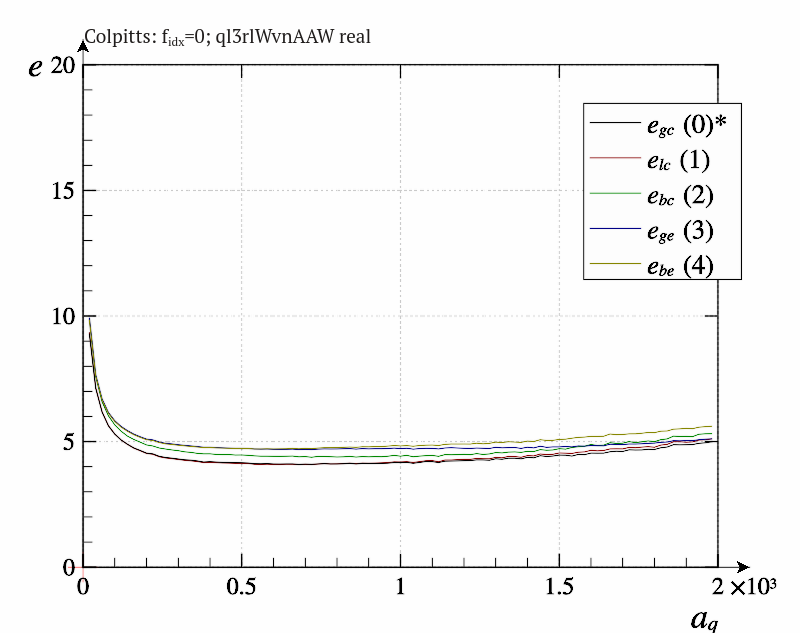
\includegraphics[width=0.50\textwidth]{p/r/colp_real_id-p_a_q_d_0.png} }
\caption{Залежності $\overline{e} (a_q) $ при ідентифікації параметра $ R_c $ генератора Колпітца за умов \ref{atu:eq:colp_test1_cond}}
\label{atu:f:colp_real_id_p_a_q_d_0}
\end{figure}

Вид цих залежностей цілком звичний для розглянутих систем
ідентифікації, і положення мінімуму похибки цілком узгоджується
з спектрами системи, що спостерігалися.

На рис.~\ref{atu:f:colp_real_id_p_q_gamma_d_0} відображені отримані залежності
$\overline{e}_{q_\gamma} $ для процесів ідентифікації параметра
$R_c $ генератора Колпітца.

\begin{figure}[htb!]
  \centerline{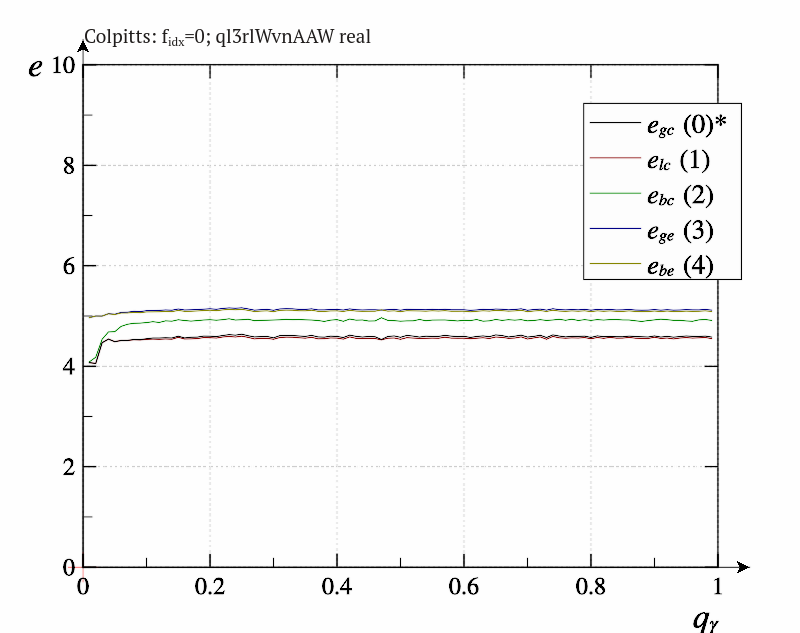
\includegraphics[width=0.50\textwidth]{p/r/colp_real_id-p_q_gamma_d_0.png} }
\caption{Залежності $ \overline{e} (q_\gamma) $ при ідентифікації параметра $ R_c $ генератора Колпітца за умов \ref{atu:eq:colp_test1_cond}}
\label{atu:f:colp_real_id_p_q_gamma_d_0}
\end{figure}

Отримані залежності мають досить дивний вигляд. Початкова
ділянка, на якої зазвичай спостерігається зростання похибки
ідентифікації через надмірну чутливість, замаскований істотним
рівнем статичної похибки ідентифікації. Подальша слабка
залежність аналогічна отриманим залежностям для інших систем.

З урахуванням цих причин залежність
$\overline{e}_{v_f} $, представлена на рис.~\ref{atu:f:colp_real_id_p_v_f_d_0},
виявляється цілком очікуваною. Динаміка агентів призводить
до їх зміщення в точку, в якій збігаються значення критеріїв
моделі і об'єкта, що, в даних умовах, призводить до зростання
похибки ідентифікації.

\begin{figure}[htb!]
  \centerline{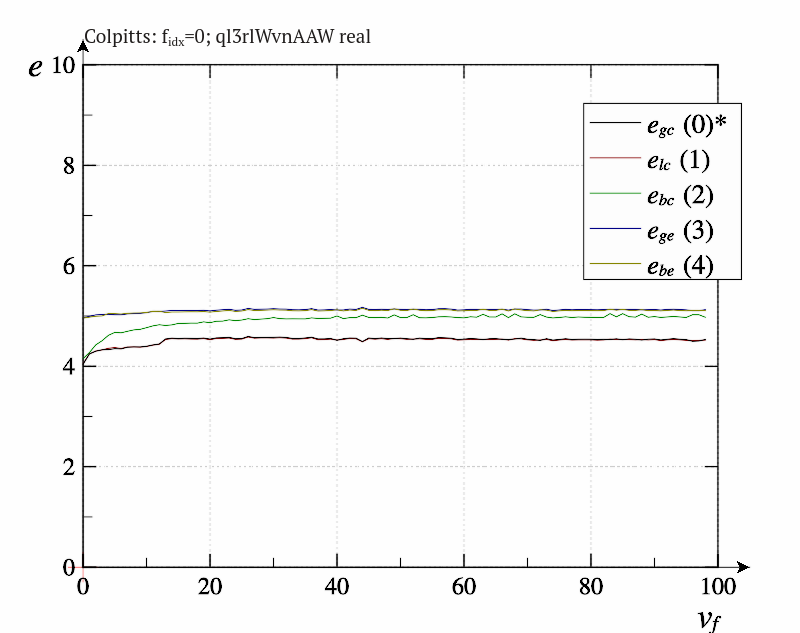
\includegraphics[width=0.45\textwidth]{p/r/colp_real_id-p_v_f_d_0.png} }
\caption{Залежності $ \overline{e} (v_f) $ при ідентифікації параметра $ R_c $ генератора Колпітца за умов (\ref{atu:eq:colp_test1_cond})}
  \label{atu:f:colp_real_id_p_v_f_d_0}
\end{figure}

Залежність
$\overline{e}_{k_e} $, що представлена на рис.~\ref{atu:f:colp_real_id_p_k_e_d_0},
абсолютно аналогічна попередній, і з тих же самих причин.

\begin{figure}[htb!]
  \centerline{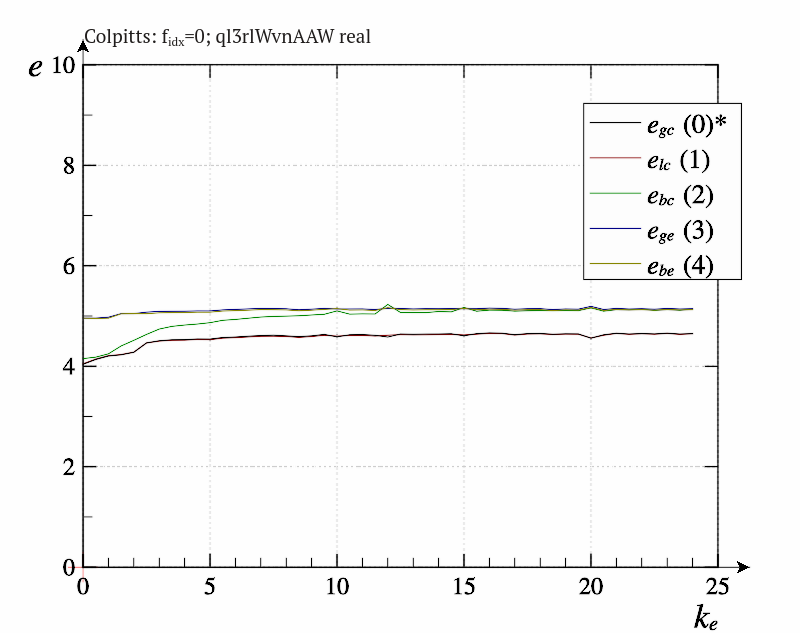
\includegraphics[width=0.45\textwidth]{p/r/colp_real_id-p_k_e_d_0.png} }
\caption{Залежності $ \overline{e} (k_e) $ при ідентифікації параметра $ R_c $ генератора Колпітца за умов (\ref{atu:eq:colp_test1_cond})}
\label{atu:f:colp_real_id_p_k_e_d_0}
\end{figure}

Залежність
$\overline{e}_{k_{nl}} $, що представлена рис.~\ref{atu:f:colp_real_id_p_k_nl_d_0},
відображає те, що обмеження індивідуальної динаміки агентів
на користь динаміки ансамблю як цілого, в даному випадку трохи
знижує похибку ідентифікації.

\begin{figure}[htb!]
  \centerline{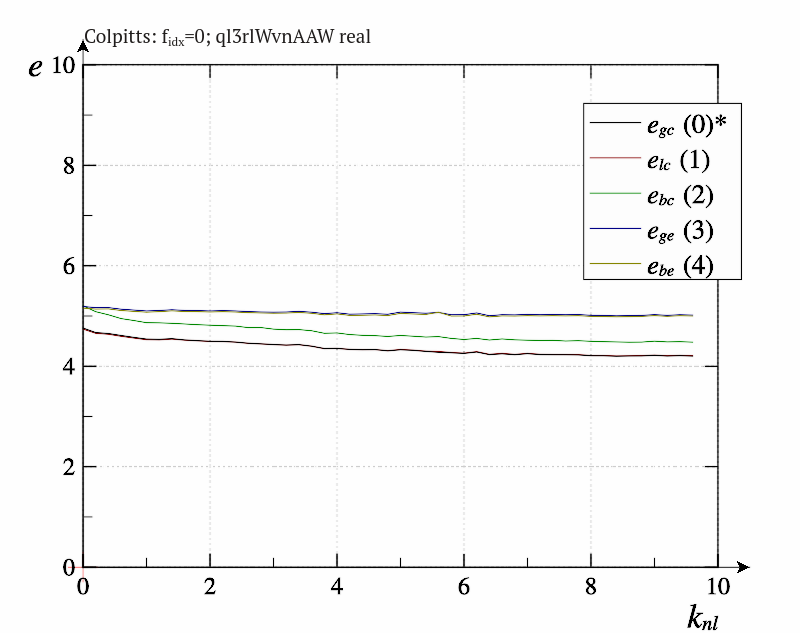
\includegraphics[width=0.45\textwidth]{p/r/colp_real_id-p_k_nl_d_0.png} }
\caption{Залежності $ \overline{e} (k_{nl}) $ при ідентифікації параметра $ R_c $ генератора Колпітца за умов (\ref{atu:eq:colp_test1_cond})}
  \label{atu:f:colp_real_id_p_k_nl_d_0}
\end{figure}
%
%
% \begin{figure}[htb!]
%   \centerline{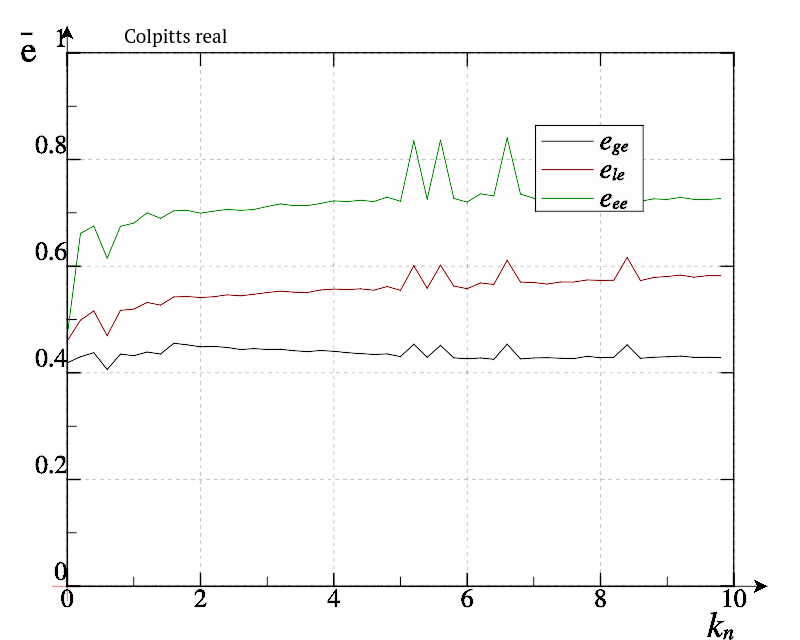
\includegraphics[width=0.6\textwidth]{p/colp_real_id_qi_fv5_prm_0-p_k_cn.png} }
%   \caption{Залежності $\overline{e}_{r*}(c_n)$ при идентификации параметра $R_c$ генератора Колпитца}
%   \label{atu:f:colp_real_id_qi_fv5_prm_0-p_k_cn.png}
% \end{figure}

В цілому, наявність статичної похибки ідентифікації, зумовленою
не повністю адекватним моделюванням, нівелює, в розумних межах,
більшу частину з розглянутих залежностей.


% }}}1


\section{Висновки по розділу \thechapter} %{{{1

Результати натурних експериментів, моделювання систем, що
описують динаміку генератора Колпітца, процесів ідентифікації
параметра
$R_c $, що визначає вид цієї динаміки, дозволяють зробити наступні
висновки:

\begin{itemize}

  \item
    Застосування для опису поведінки генератора Колпітца
    класичної моделі виду (\ref{atu:eq:colp}) дозволяє отримати тільки
    якісну подобу. Ця модель відображає наявність режимів, що
    спостерігаються у реальної системи, і переходів між ними. Однак,
    і форма коливань, і параметри переходу дотримуються дуже
    приблизно.

  \item
    Для класичної моделі можлива побудова системи ідентифікації
    параметра
    $b$ з використанням ансамблю агентів і критерію
    $q_{x^2} $.

  \item
    Використання уточненої моделі генератора Колпітца, із
    застосуванням опису транзистора виду~(\ref{atu:eq:bjt_model_sub}) дозволяє
    точніше описати динаміку.

  \item
    На відміну від класичної моделі, при ідентифікації уточненої
    має сенс застосовувати критерій
    $q_{xz} $ замість
    $q_{x^2} $. При цьому спостерігається відмінність між значеннями
    цього критерію для моделі та об'єкту близько~5\%.

  \item
    Метод ідентифікації параметра
    $R_c$ реального об'єкта ансамблевим методом з використанням
    критерію
    $q_{xz}$ виявився працездатним. При цей основний внесок в похибку
    ідентифікації вносить відмінність між значеннями критерію
    реального об'єкта і відповідної йому моделі.

  \item
    Наявність помітною статичної похибки ідентифікації робить
    настройку параметрів системи ідентифікації менш виправданою.

\end{itemize}


В цілому синтез критерію ідентифікації та побудова працездатною
системи ідентифікації для системи генератора Колпітца
не вимагає ніяких спеціальних підходів і введення
додаткових заходів оцінювання взаємозв'язків параметрів
генератора.

Список використаних джерел у даному розділі наведено у повному
списку використаних джерел під номерами
\cite{atu_apir2013},
\cite{atu_st104a},
\cite{DBLP:journals/corr/WangWQ15},
\cite{dmitriev_gen_chaos},
\cite{doi:10.1063/1.4705999},
\cite{gummel_poon_1970},
\cite{shiskin_electronnie_pribori},
\cite{horowitz},
\cite{kennedy_chaos_colpitts},
\cite{atu_asau21},
\cite{Kennedy_Colpitts_predicting},
\cite{Kennedy_Colpitts_Chua},
\cite{PhysRevE.80.016201},
\cite{picovskii_syncro},
\cite{bonetti_super_persistent_colpitts},
\cite{zaeplnii_radio_calc}.

% }}}1

% vim: fdm=marker foldlevel=0 foldignore="%#" fdc=4 ft=tex
